\section{Some discussion}

This chapter will concern most of the numerical error analysis and some of the discussion of this analysis as well as an introduction to the methods used for error analysis in general, and how they are adapted to this particular problem.\\


In this numerical setup we will potentially introduce several new error sources in addition to the normal errors introduced by numerical solution of any equation (see section \ref{some_words_on_PDEs}). 
When a part of the solution acquired is replaced by the solution from another model, which in this case is stochastic, we will change the initial condition to the next iteration in time. 
This might have a number of effects on our final solution. 
When we solve a differential equation numerically we only get an approximation to the actual solution because we are using approximate derivatives (see figure \ref{illustrate_approximate_derivatives}). 
To investigate the error we are introducing we will first need to test that the truncation error of the numerical PDE solver behaves as expected. 
% This can be done by choosing a solution to the PDE, doing a simulation which should yield the same solution and then comparing the two answers. 
% As argued in section \ref{} we will struggle with making the error from the random walk solver be much smaller than $\mathcal{O}(\Delta t)$. 
% We will therefore start by using a simple discretization of the PDE which also has a truncation error of $\mathcal{O}(\Delta t)$. 
% Figure \ref{errorplot_1d} shows the error norm (\ref{}) of only the PDE solver done in 1 dimension plotted for each timestep of the simulation. 
% The manufactured, exact solution is $u(x,t) = \exp\left(-\pi^2t\right)\cos(\pi x)$ and its initial condition is shown in figure \ref{}.

\begin{figure}[H]
 \centering
%  \includegraphics[scale=0.7]{/home/fredriep/Dropbox/uio/thesis/doc/results/experiment_31102013_1017/results/initial_condition.eps}
 \includegraphics[scale=0.7]{../doc/results/experiment_31102013_1017/results/initial_condition.eps}
 \caption[Initial condition in 1d]{Initial condition of manufactured solution in 1d and the simulation.}
 \label{initial_condition_1d}
\end{figure}

\subsection{The error estimate}
Before we do anything we should specify what we use to measure the error. 
Throughout this thesis the term error is used quite lazily, but except something else is specified we refer to the expression 
\begin{equation}
 err = max\left(||u_e-u||_2\right)
\end{equation}
where $u_e$ is the exact (manufactured) solution to the equation. 
This is not necessarily the best error measure, but as it lets us study the time evolution of the error it makes debugging a bit simpler. 
Other error measures that might come in handy later will be the integrated spatial error as a function of time
\begin{equation}
 err = ||\sum u_e-u||_2
\end{equation}
and the same error integrated in time as well
\begin{equation}
 err = \sum||\sum u_e-u||_2
\end{equation}
The error will be calculated over the entire mesh, regardless of any random walk areas on the mesh.

\section{Manufactured Solutions}
A normal way of checking that our scheme of choice is implemented correctly is by making an exact solution to the equation and checking that the error is of the expected order. 
As a first, simple implementation we have worked with the explicit Forward Euler discretization of the simplest form of the diffusion equation \ref{simple_diffusion_equation}. 
This discretization is expected to have an error-term of the order of $\Delta t$, which again is limited by a stability criterion. 
We can now decide that the solution to equation \ref{simple_diffusion_equation} should be
\begin{equation}\label{manifactured_solution_1D}
 u(x,t) = e^{-t\pi^2}\cos(\pi x) +1
\end{equation}
which satisfies our equation if we set the diffusion constant to 1.
\begin{align}
 \frac{\d }{\d t}e^{-t\pi^2}\cos(\pi x) +1 &= D\frac{\d^2}{\d x^2}e^{-t\pi^2}\cos(\pi x) +1\\
 -\pi^2e^{-t\pi^2}\cos(\pi x) &= -\pi^2e^{-t\pi^2}\cos(\pi x) +1 \implies 1 = 1
\end{align}
As we saw in section \ref{truncation_error} the Forward Euler scheme is expected to have an error of the order of $\Delta t$ in time. 
The error in space is determined by two factors, the actual error caused by the approximation to the second derivative, which is of the order of $\Delta x^2$ and the error term coming from the time derivative due to the stability criterion \ref{stability}, which is also of the order $\Delta x^2$. 
Testing only the scheme first, in 1D we get the following plot \ref{errorplot_FE1D_noWalk} of the maximum of the absolute value of the difference between the exact solution and the numerical solution to the equation, showing us that the error is linear in the first part of a simulation. 
For longer simulations, however, we expect the analytic solution to take a steady state which we find in the limit of large $t$. 
\begin{equation}
 u(x,t\to\infty) \to e^{-\infty}\cos(\pi x) +1 \to 1
\end{equation}
The numerical scheme should be able to represent this to machine precision ($10^{-16}$), meaning that the numerical solution should start converging to zero after some number of times steps. 
Figure \ref{errorplot_FE1D_noWalk_long} shows a longer simulation of the equation which includes the converging part as well. 
Looking closely at figure \ref{errorplot_FE1D_noWalk_long}, which has a smaller $\Delta t$ by a factor of $\sim6$ with respect to figure \ref{errorplot_FE1D_noWalk}, we can note that the error norm $0.0015$ is reached after some $100-200$ time steps, which is later than in figure \ref{errorplot_FE1D_noWalk}. 
Although this is not an exact measurement, it is another indication that the implementation is correct.

\begin{figure}[H]
\centering
\begin{subfigure}[b]{0.48\textwidth}
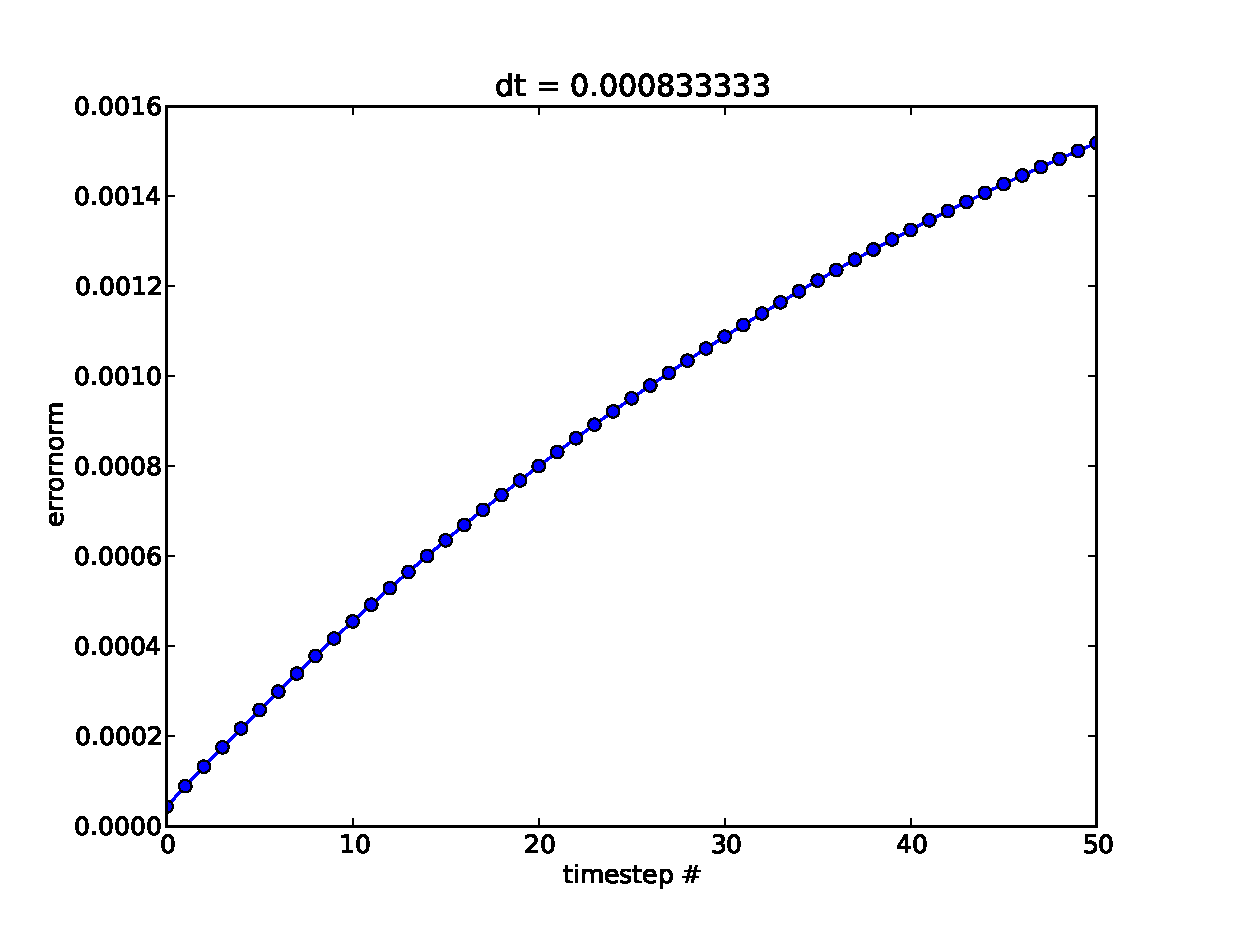
\includegraphics[width=\textwidth]{../doc/results/experiment_31102013_1017/results/deterministic_errorplot.eps}
\caption{}
\label{errorplot_FE1D_noWalk}
\end{subfigure}
\begin{subfigure}[b]{0.48\textwidth}
 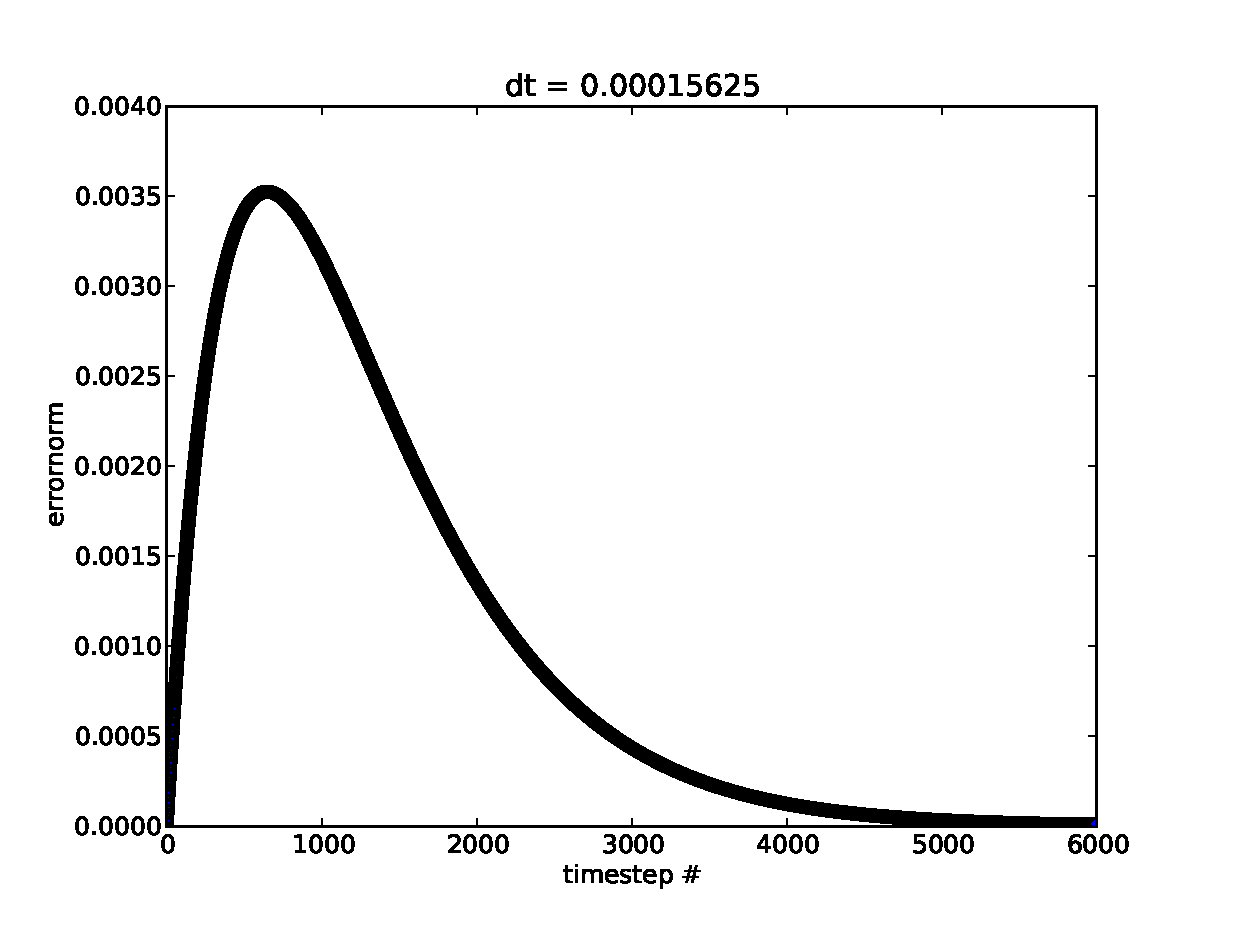
\includegraphics[width=\textwidth]{../doc/results/experiment_18112013_0830/results/deterministic_errorplot.eps}
 \caption{}
 \label{errorplot_FE1D_noWalk_long}
\end{subfigure}
\caption[Numerical error for 1D Forward Euler discretization]{Numerical error for 1D Forward Euler discretization of the PDE. Nothing else is done to the simulation.}
\label{errorplot_FE1D_noWalk_super}
\end{figure}

We then introduce an area on the domain where we switch models from the normal PDE to an average of the PDE solution and the result of a random walk simulation where the initial condition is the last time step from the PDE converted to walkers by the conversion rate given in equation \ref{conversion_rate}. In this case we have used the parameters $a=3$, $\Delta t = \frac{\Delta x^2}{3.0}$, $\Delta x = \frac{1}{20}$. 
These parameters makes one unit of $u(x,t)$ equal to some $1000$ walkers. 
\begin{equation}\label{conversion_rate}
 C_{ij} = \frac{a}{\Delta t}U_{ij}
\end{equation}
Mostly we will rewrite equation \ref{conversion_rate} to just one conversion factor times the PDE solution, giving us some flexibility should we want to add more dependencies in the conversion. 
As of now, the conversion factor, $Hc$, is defined in equation \ref{definition_Hc_first}. 
One ``unit'' of $ U_{ij}$ will directly correspond to $Hc$ random walkers.
\begin{equation}\label{definition_Hc_first}
 Hc =  \frac{a}{\Delta t} \implies C_{ij} = Hc\cdot U_{ij}
\end{equation}

The area where the model has been replaced is between $x=0.6$ and $x=0.7$, which is three mesh points. 
In the same way as for only the simple 1D PDE case we compare the combined numerical solution from the two models to the exact solution. 
Figure \ref{errorplot_FE1D_Walk_first_attemt} shows that the error is still of the order of $\Delta t$, and the difference between the two models are negligible. 

\begin{figure}[H]
\centering
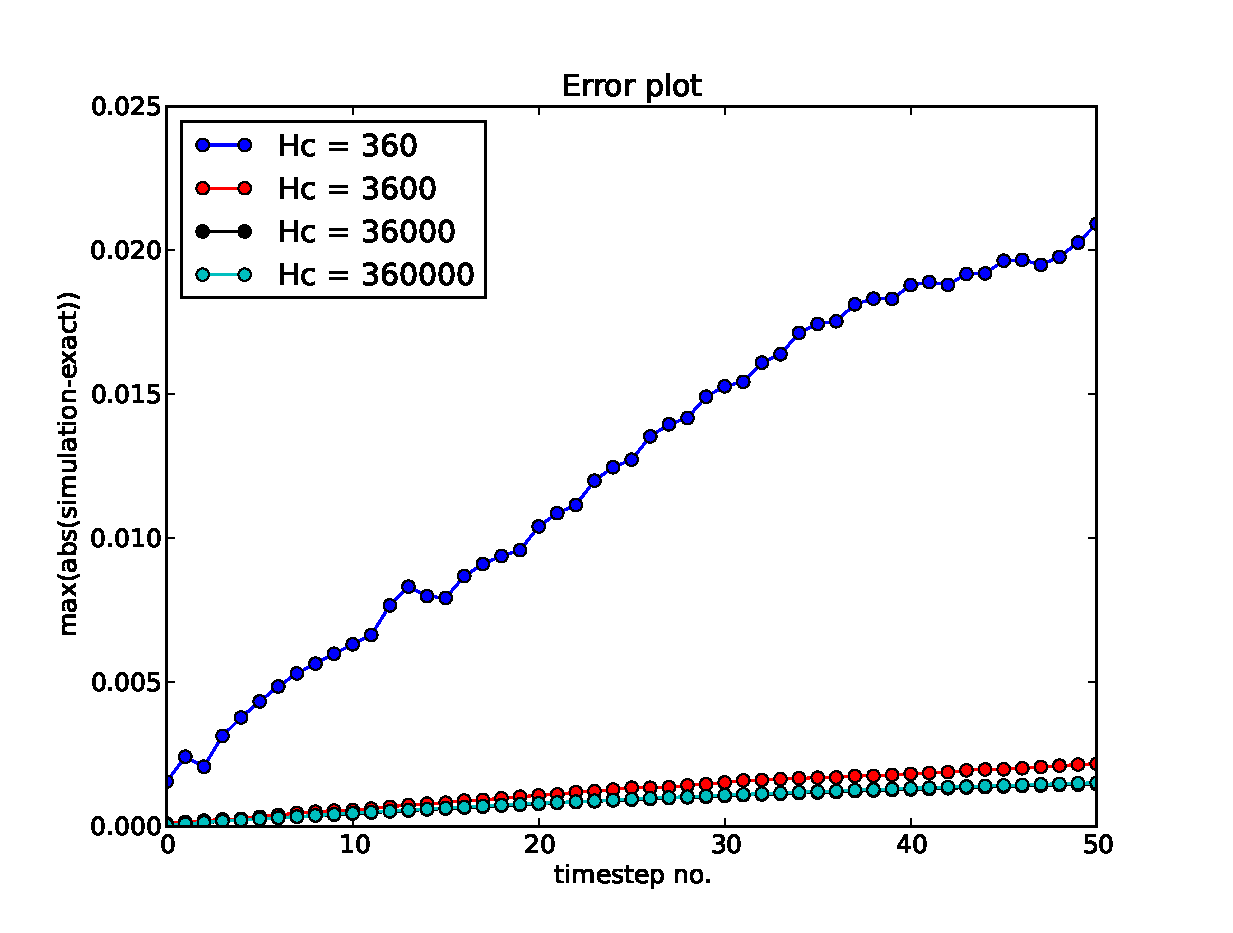
\includegraphics[scale=0.7]{../doc/results/experiment_31102013_1017/results/errorplot.eps}
\caption[Effect of increasing number of walkers]{Numerical error for 1D Forward Euler discretization combined with random walk model between $x=0.6$ and $x=0.7$. Other parameters of importance are $\Delta t\approx 0.00083333$, $\Delta x = 0.05$.}
\label{errorplot_FE1D_Walk_first_attemt}
\end{figure}

As we can see from figure \ref{errorplot_FE1D_Walk_first_attemt} increasing the number of walkers that each ``unit concentration'' corresponds to has a positive effect on the error norm up to a certain point. 
After we reach $Hc \sim 10^4$ the error is dominated by the truncation error of the Forward Euler scheme. 
This tells us that the error associated with introducing a random walk model on parts of the mesh behaves roughly as we hoped; it tends to zero for large numbers of walkers. 
Meaning of course that the calculations in section \ref{} are not hopeless.

We can also do a convergence test to see that the error is approximately of the expected order. 
This is done by doing several simulations with different values for $\Delta t$ and comparing the errors by equation \ref{convergence_rate_def}. 
A result of such an experiment for the FE scheme using the $\Delta t$ values listed below is found in figure \ref{convergence_test_FE}. 
The expected value of r is approximately 1. The result is not perfect, but still close to 1.
\begin{lstlisting}
 dt = [1e-4,1e-5,1e-6,1e-7,1e-8]
\end{lstlisting}
\begin{figure}[H]
 \centering
 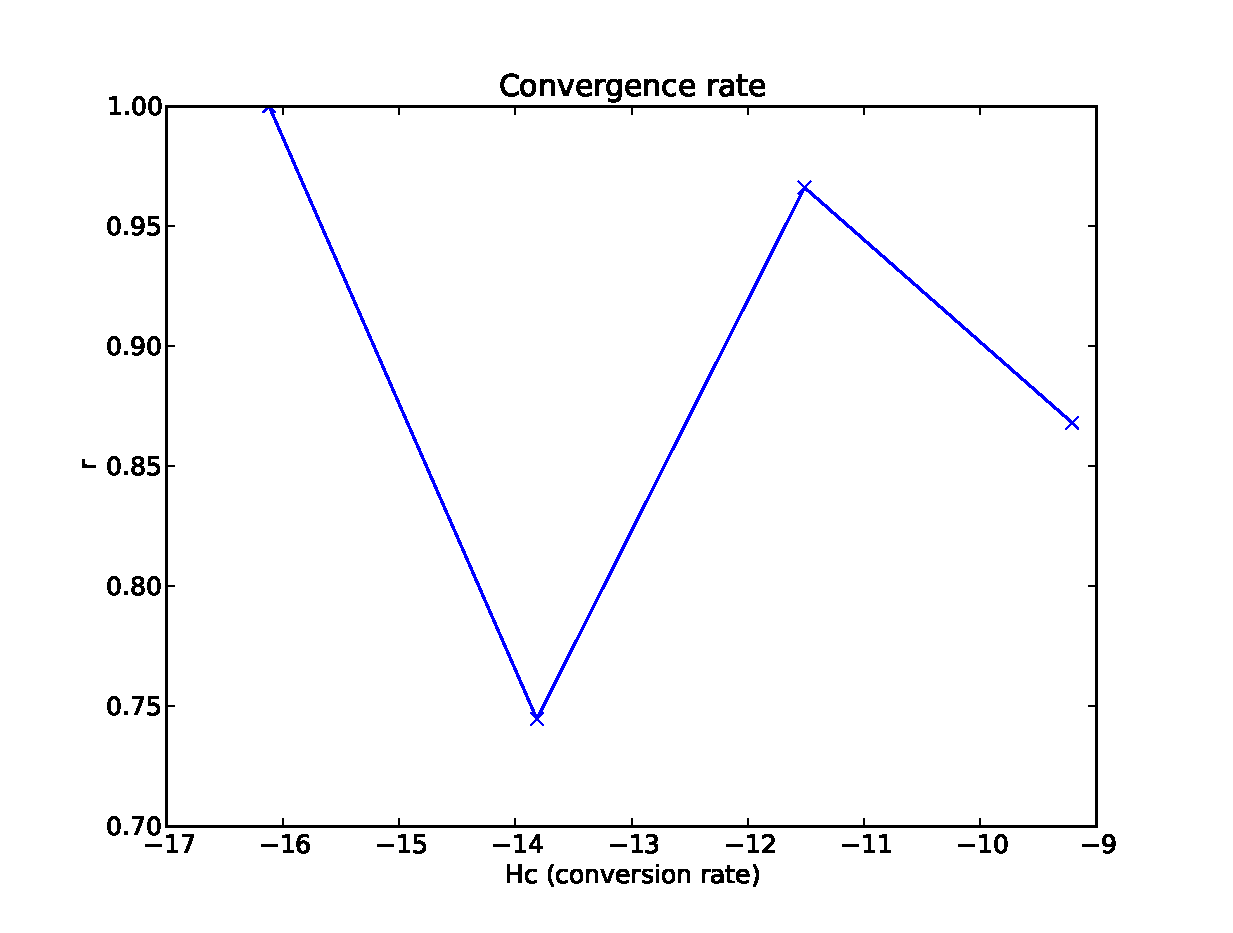
\includegraphics[scale=0.7]{../doc/results/experiment_27112013_1017/results/ConvergenceTest.eps}
 \caption{Convergence test for the FE scheme. The x axis is $\ln(\Delta t)$.}
 \label{convergence_test_FE}
\end{figure}



\subsection{Exact numerical solution}

The FE scheme also has an exact solution seeing as it is in fact a difference equation. 
We can find this (for this exact initial condition \ref{initial_condition_1d}) if we formulate the scheme as 

\begin{equation}
 u^{n+1} = D\Delta t u_{xx}^n + u^n
\end{equation}

and insert for the first few iterations. 

\begin{align*}
 u^1 &= D\Delta t u_{xx}^0 + u^0 \\
 u^2 &= D\Delta t u_{xx}^1 + u^1 = D\Delta t\left[D\Delta t u_{4x}^0 + u_{2x}^0\right] + u^0\\
 &= \left(D\Delta t\right)^2 u_{4x}^0 + 2D\Delta t u_{2x}^0+ u^0 \\
 u^3 &= D\Delta t u_{xx}^2 + u^2 = D\Delta t\left[\left(D\Delta t\right)^2 u_{6x}^0 + 2D\Delta t u_{4x}^0+ u_{2x}^0\right] + \left(D\Delta t\right)^2 u_{4x}^0 + 2D\Delta t u_{2x}^0+ u^0\\
 &= \left(D\Delta t\right)^3 u_{6x}^0 + 3\left(D\Delta t\right)^2 u_{4x}^0+ 3D\Delta tu_{2x}^0 + u^0 \\
 u^4 &= D\Delta t u_{xx}^3 + u^3 = \dots \\
 &= \left(D\Delta t\right)^4 u_{8x}^0 + 4\left(D\Delta t\right)^3 u_{6x}^0+ 6\left(D\Delta t\right)^2 u_{4x}^0 + 4D\Delta t u_{2x}^0 + u^0 
\end{align*}
Which we can generalize to 
\begin{equation}
 u^{n+1} = \sum\limits_{i=0}^n {n\choose i}\left(D\Delta t\right)^iu^0_{2ix}
\end{equation}
where we have
\begin{equation*}
 u^0_{2ix} = \left(-1\right)^i\pi^{2i}\cos(\pi x)
\end{equation*}
from the initial condition. This finally gives us the exact numerical solution of the FE scheme in time. 
\begin{equation}
 u^{n+1} = \sum\limits_{i=0}^n {n\choose i}\pi^{2i}\left(-1\right)^i\left(D\Delta t\right)^i\cos(\pi x)
\end{equation}
Notice that we have not used the approximation to the spatial derivative, but rather the analytical derivative. 
We can find the approximation that the computer uses to the spatial derivative in the same way as for the time derivative. 
\begin{align*}
 u^0_{xx} &= \frac{1}{\Delta x^2}\left(\cos(\pi(x+\Delta x)) -2\cos(\pi x) +\cos(\pi(x-\Delta x))\right) \\
 &= \frac{2}{\Delta x^2}\left(\cos(\pi\Delta x)-1\right)\cos(\pi x)\\
 u^0_{4x} &= [u^0_xx]_{xx} = \frac{1}{\Delta x^2}\left[\frac{2}{\Delta x^2}\left(\cos(\pi\Delta x)-1\right)\left(\cos(\pi(x+\Delta x)) -2\cos(\pi x) +\cos(\pi(x-\Delta x))\right)\right]\\
 &= \frac{4}{\Delta x^2}\left(\cos(\pi\Delta x)-1\right)^2\cos(\pi x)\\
 &\dots
\end{align*}
We can immediately see that this pattern continues, and we get the general formula in equation \ref{numerical_solution} for the exact numerical solution.
\begin{equation}\label{numerical_solution}
  u^{n+1} = \sum\limits_{i=0}^n {n\choose i}\left(D\Delta t\right)^i\frac{2^i}{\Delta x^{2i}}\left(\cos(\pi\Delta x)-1\right)^i\cos(\pi x)
\end{equation}
We expect the FE scheme to represent this solution more or less to machine precision, at least to $15$ digits. 
There are, however two issues with the solution \ref{numerical_solution}:
\begin{itemize}
 \item $\Delta x^{2i}$ will quickly tend to zero, and the computer will interpret it as zero. This will cause division by zero, which again ruins the simulation. This can be fixed rather simply by testing if $\Delta x^{2i}>0$ and returning zero if the test returns false.
 \item ${n\choose i}$ goes to infinity for large n and i. We will eventually (for $n>\sim170$) meet overflow. Figure \ref{convergence_exact_numerical_1d_n145} shows that at least for relatively few time steps  we can drop the troublesome terms.
\end{itemize}

\begin{figure}[H]
 \centering
 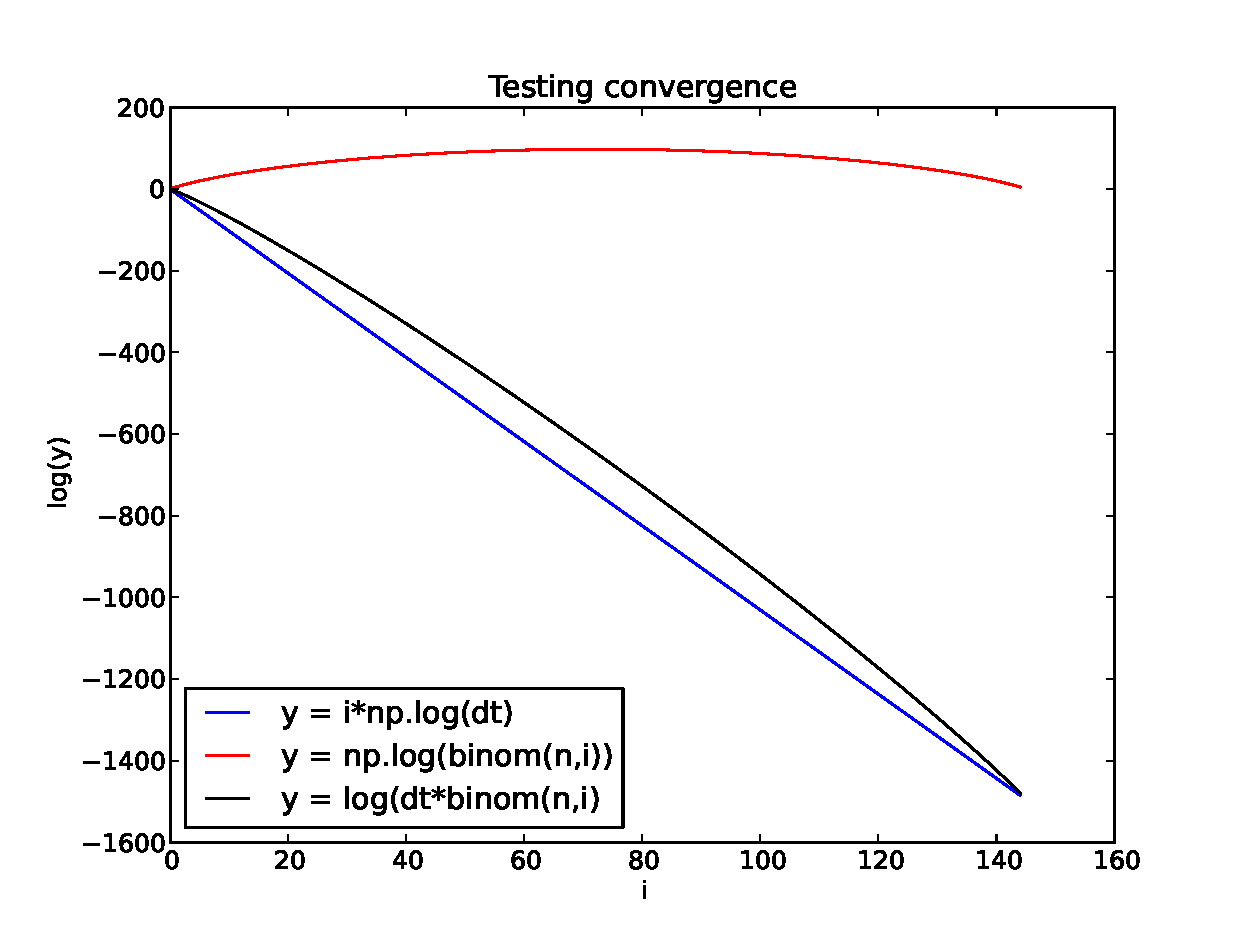
\includegraphics[scale=0.7]{Figures/convergence_exact_numerical_1d_n145}
 \caption{Testing the relation between $\left(D\Delta t\right)^i$ and the binomial coefficients.}
 \label{convergence_exact_numerical_1d_n145}
\end{figure}
The results from testing the FE scheme are found in figure \ref{errorplot_numerical_exact_FE_1D}. We see that the error in the worst case is about an order of magnitude worse than we expected. This is most likely due to the fact that we are cutting part of the solution, and over several time steps the error we do might accumulate.

\begin{figure}[H]
 \centering
 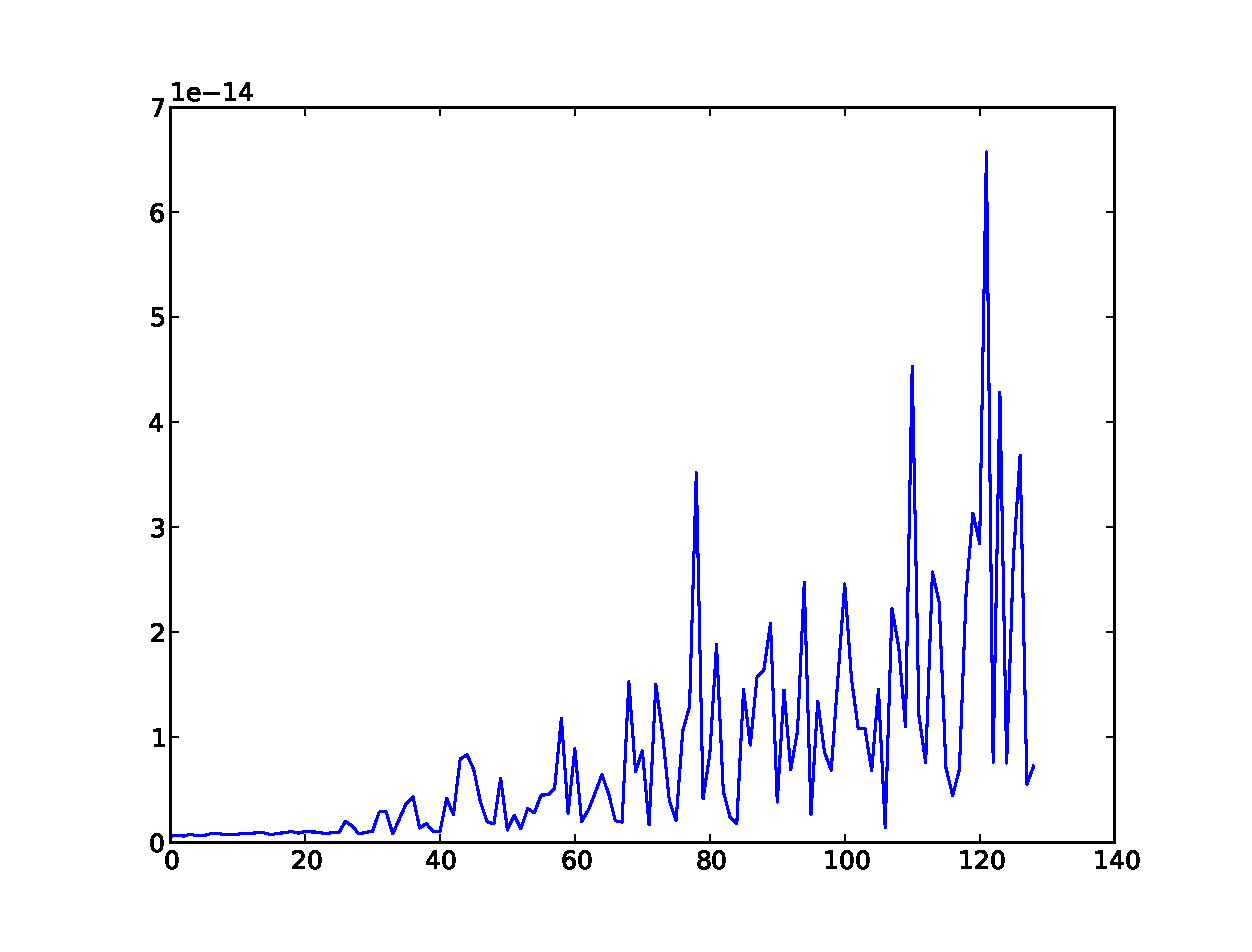
\includegraphics[scale=0.7]{Figures/exact_numerical_1d_n130.eps}
 \caption[Verification for exact numerical solution]{Error plot for 1d FE scheme compared to the exact numerical solution \ref{numerical_solution} with the modifications suggested earlier.}
 \label{errorplot_numerical_exact_FE_1D}
\end{figure}


\subsection{Increasing the time step and the relative size of walk-area}\label{increasing_dt}

Now that we have an estimate of how to adjust the step length of the walkers in order to adjust for the time step, $\Delta t$, on the PDE level we would like to investigate the actual effects of running the simulation with a larger time step to verify our calculations. 
First off all, figure \ref{errorplot_BE1D_noWalk} shows the error norm of a simulation of the simplest diffusion equation \ref{simple_diffusion_equation} discretized by the Backward Euler scheme \ref{BE_discretisation_isotropic} using a time step which would make the Forward Euler discretization unstable (There is something strange about its convergence). 
Figure \ref{errorplot_BE1D_Walk} shows the same simulation for various conversion parameters for the random walk. 
These simulations have input from the random walk model on some 20\% of the mesh points. 
As a comparison we can turn to figures \ref{errorplot_BE1D_walk_5_percent} and \ref{errorplot_BE1D_walk_35_percent} which have 5\% and 35\% of the mesh points affected by walkers.

\begin{figure}[H]
\centering
\begin{subfigure}[b]{0.48\textwidth}
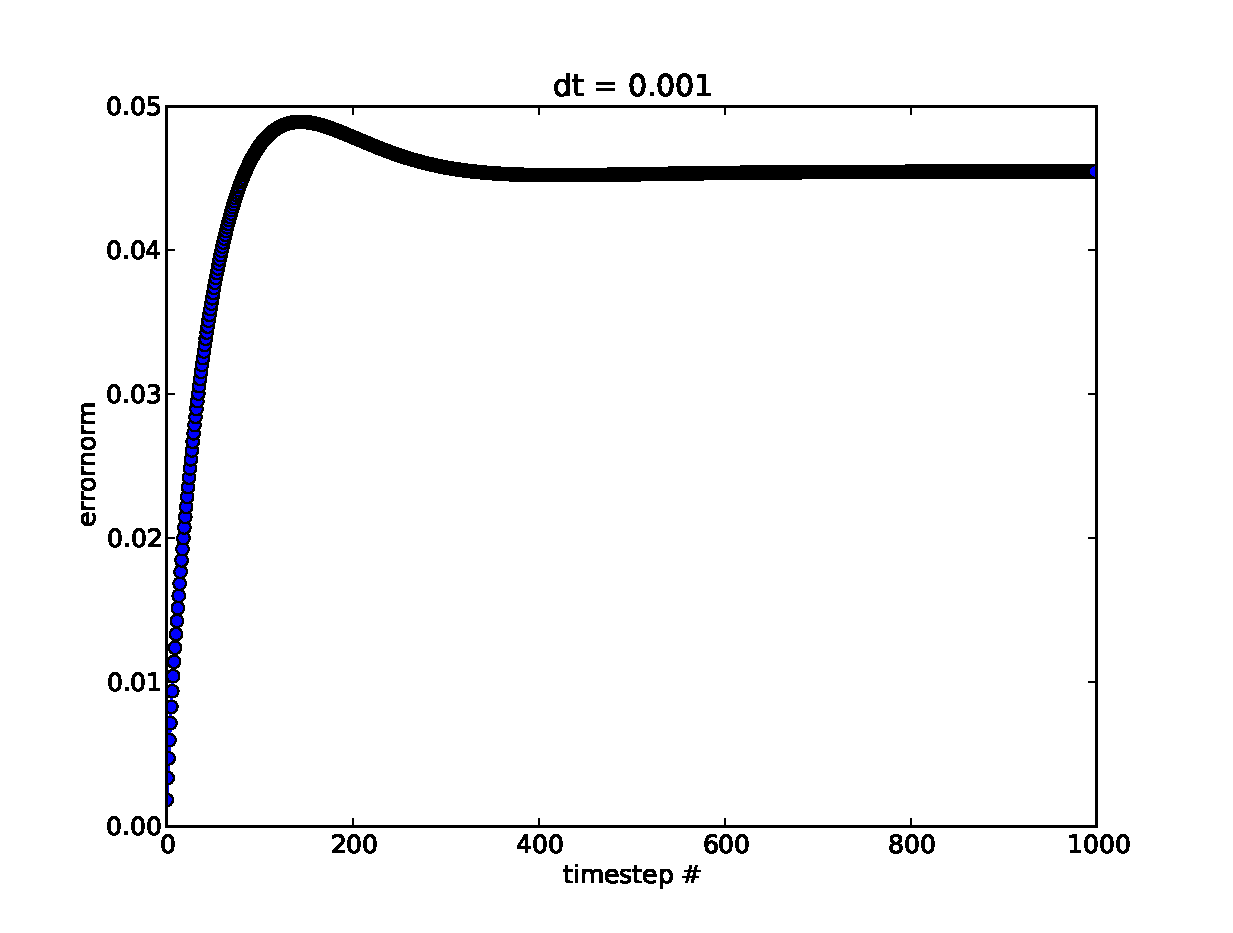
\includegraphics[width=\textwidth]{../doc/results/experiment_19112013_1514/results/deterministic_errorplot.eps}
\caption{}
\label{errorplot_BE1D_noWalk}
\end{subfigure}
\begin{subfigure}[b]{0.48\textwidth}
 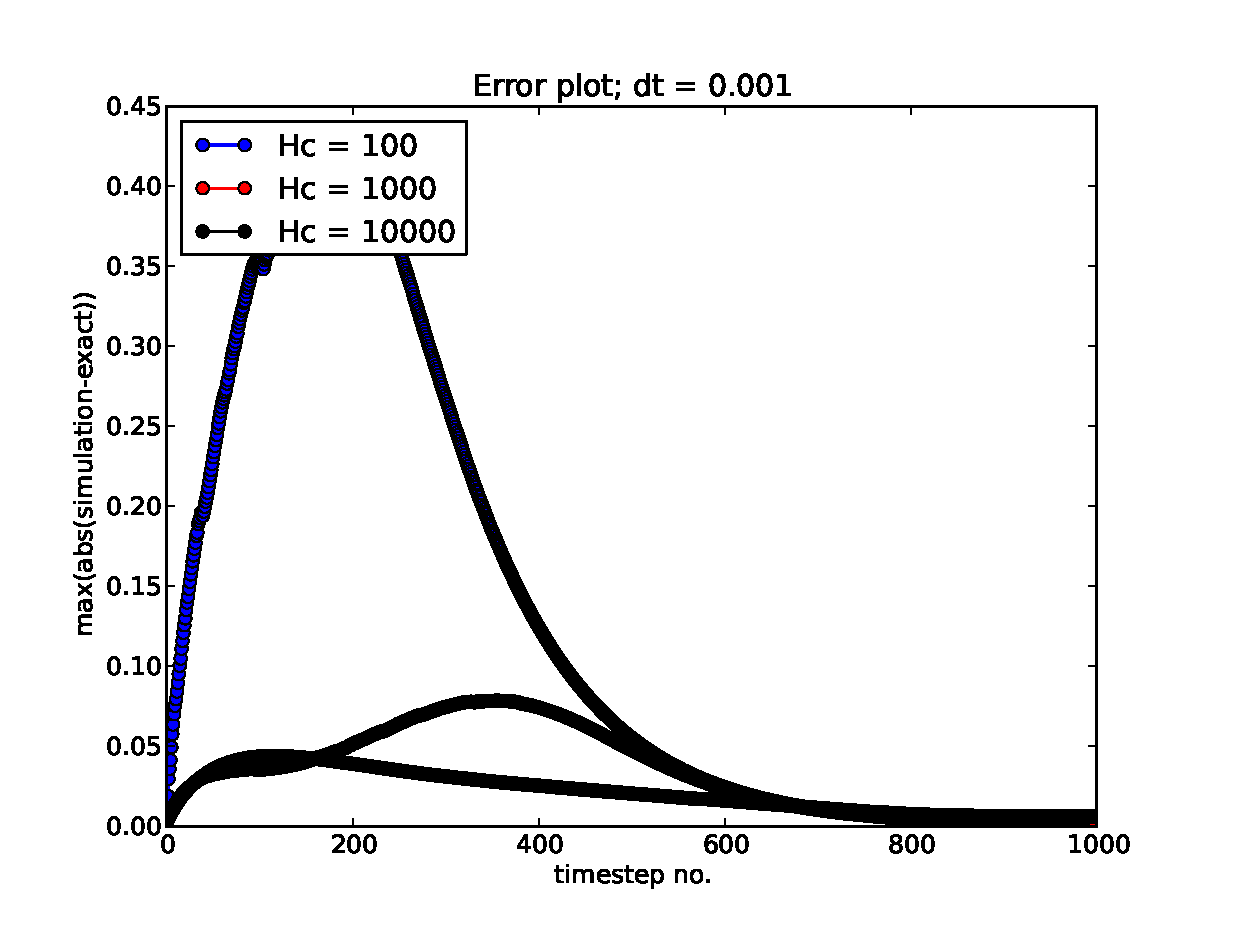
\includegraphics[width=\textwidth]{../doc/results/experiment_19112013_1514/results/errorplot.eps}
 \caption{}
 \label{errorplot_BE1D_Walk}
\end{subfigure}
\caption[Numerical error for 1D Backward Euler discretization]{Numerical error for 1D Backward Euler discretization of the PDE. In figure b there has been added walkers to the solution in the area $x\in[0.5,0.7]$.}
\label{errorplot_BE1D_first}
\end{figure}

\begin{figure}[H]
\centering
\begin{subfigure}[b]{0.48\textwidth}
 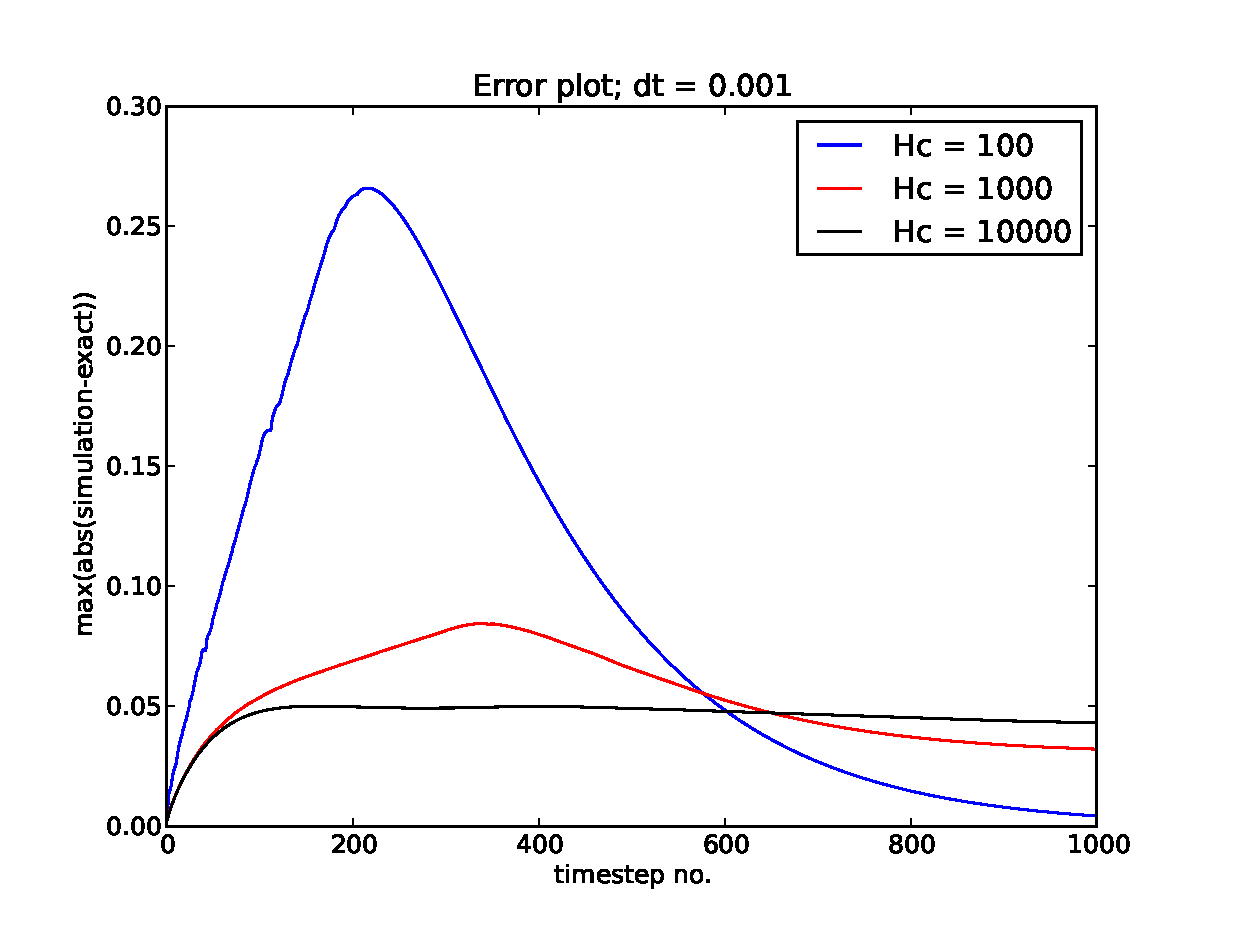
\includegraphics[width=\textwidth]{../doc/results/experiment_19112013_1559/results/errorplot.eps}
 \caption{Having walkers on 5\% of the mesh points.}
 \label{errorplot_BE1D_walk_5_percent}
\end{subfigure}
\begin{subfigure}[b]{0.48\textwidth}
 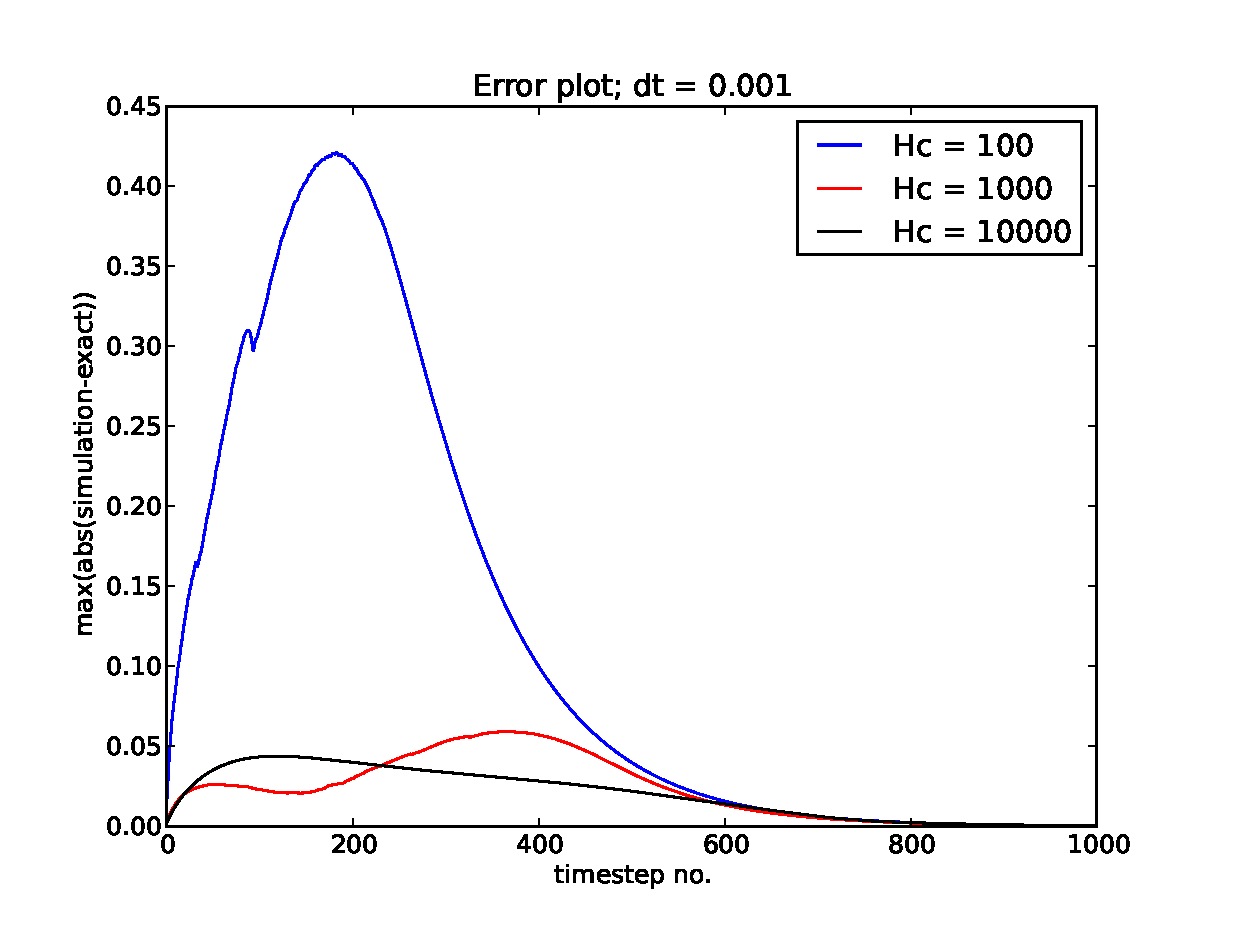
\includegraphics[width=\textwidth]{../doc/results/experiment_19112013_1603/results/errorplot.eps}
 \caption{Having walkers on 35\% of the mesh points.}
 \label{errorplot_BE1D_walk_35_percent}
\end{subfigure}
\caption{The effect of increasing the size of the walk area for a fixed $\Delta t = 0.001$ using the BE discretization.}
\label{testing_walk_area_size_BE}
\end{figure}

These experiments have been done using the Backward Euler discretization so that we can simulate for a longer time and still see the effects to their full extent. 
We have also investigated the effects of changing the time step (also using the BE discretization to avoid instabilities and be able to do longer simulations). 
The results are summarized in figure \ref{testing_dt_size}. 
We notice something a bit unexpected in figure \ref{errorplot_BE1D_walk_large_dt}. 
Unlike almost all the other comparable plots, it seems that using the least amount of walkers gives the best result here. 
This might be because the system quickly reaches its steady state, and will then be very well described by the continuum model. 
Having a small conversion factor, Hc, will mean that very quickly there will be no walkers which sort of ruins the point. 
This particular equation has steady state $u(t\to\infty,x) = 0$, and so not having any walkers will be perfect. What we should read from this figure is rather that the simulation with the most walkers converges to an acceptable error, and that this is achieved just as fast as for the other two simulations.



\begin{figure}[H]
\centering
\begin{subfigure}[b]{0.48\textwidth}
 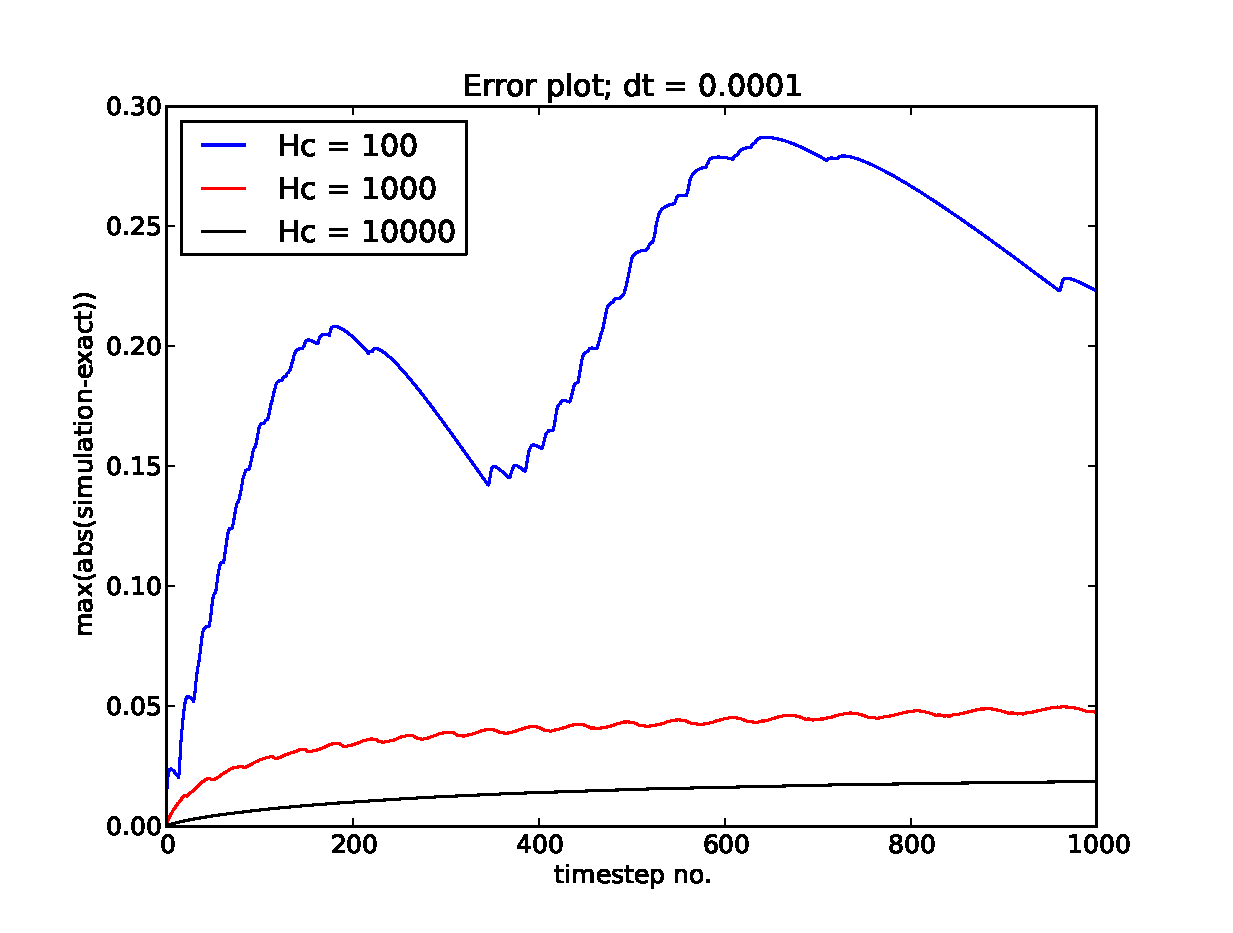
\includegraphics[width=\textwidth]{../doc/results/experiment_19112013_1625/results/errorplot.eps}
 \caption{Using a normal $\Delta t = 0.0001$.}
 \label{errorplot_BE1D_small_dt}
\end{subfigure}
\begin{subfigure}[b]{0.48\textwidth}
 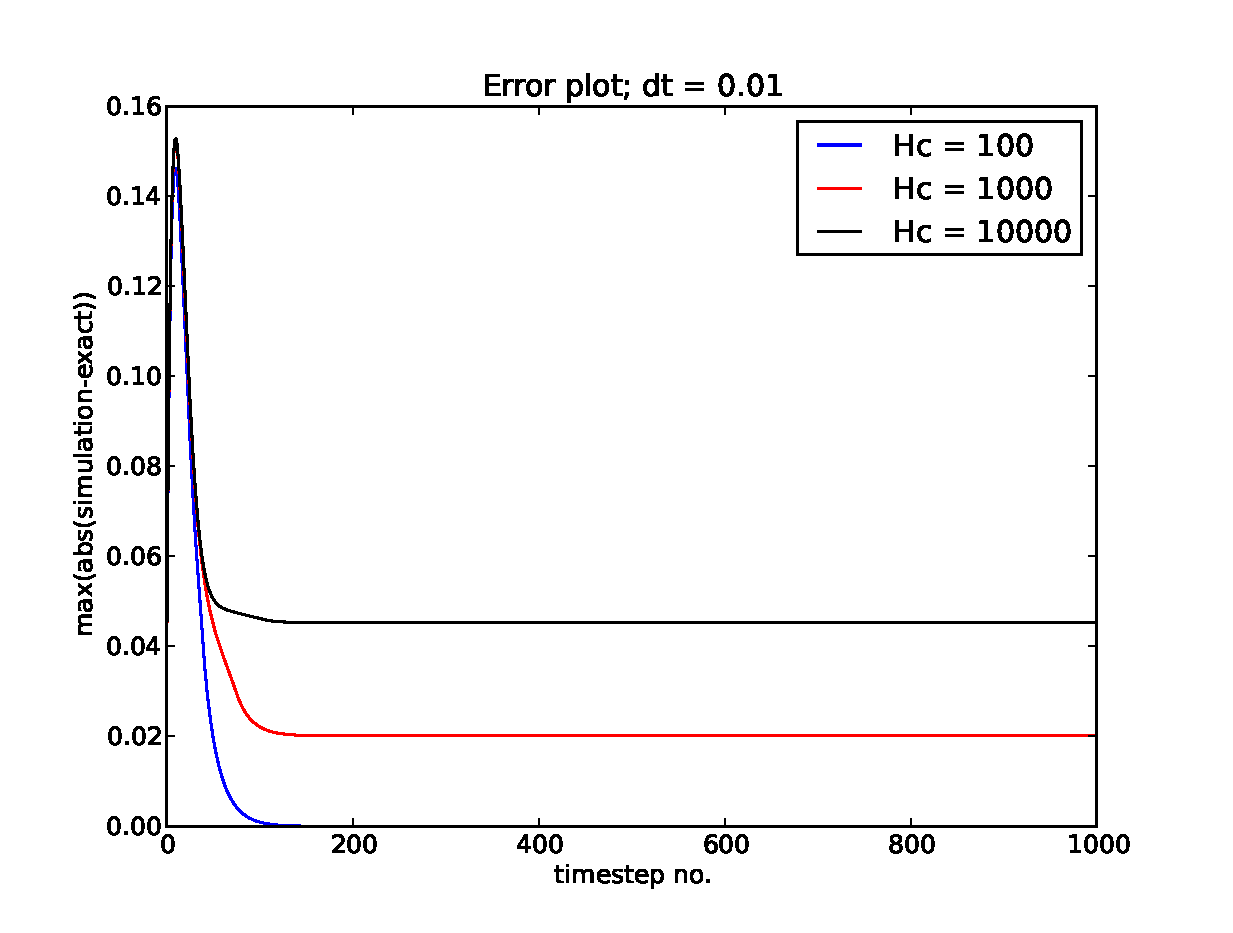
\includegraphics[width=\textwidth]{../doc/results/experiment_19112013_1627/results/errorplot.eps}
 \caption{Using a large $\Delta t = 0.01$.}
 \label{errorplot_BE1D_walk_large_dt}
\end{subfigure}
\caption{}
\label{testing_dt_size}
\end{figure}

\begin{figure}[H]
 \centering
\begin{subfigure}[b]{0.48\textwidth}
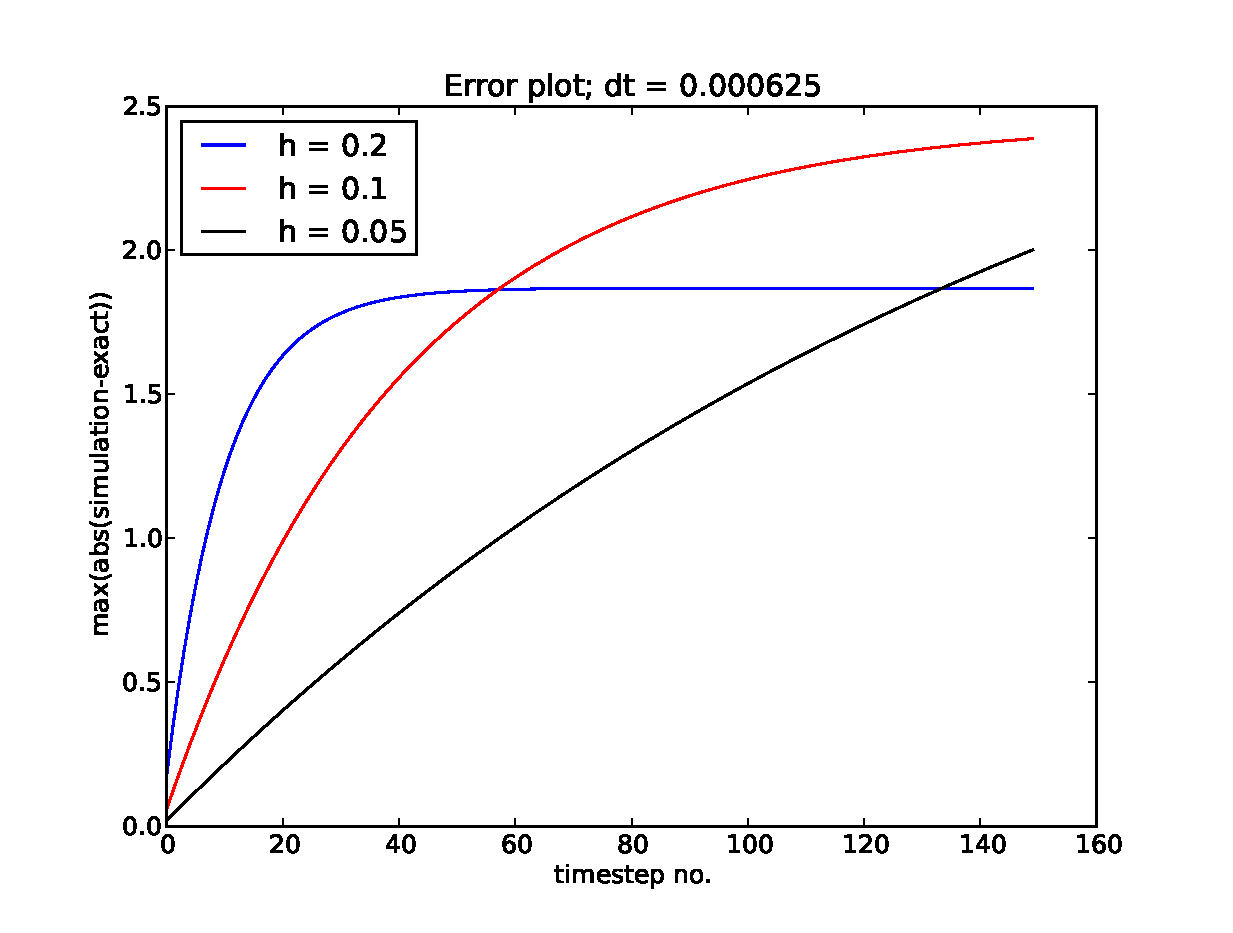
\includegraphics[width=\textwidth]{{../doc/results/experiment_02122013_1309_long_simulations_1d/results/errorplot}.eps}
 \caption{}
 \label{errorplot_FE_walk_long:normal}
\end{subfigure}
\begin{subfigure}[b]{0.48\textwidth}
 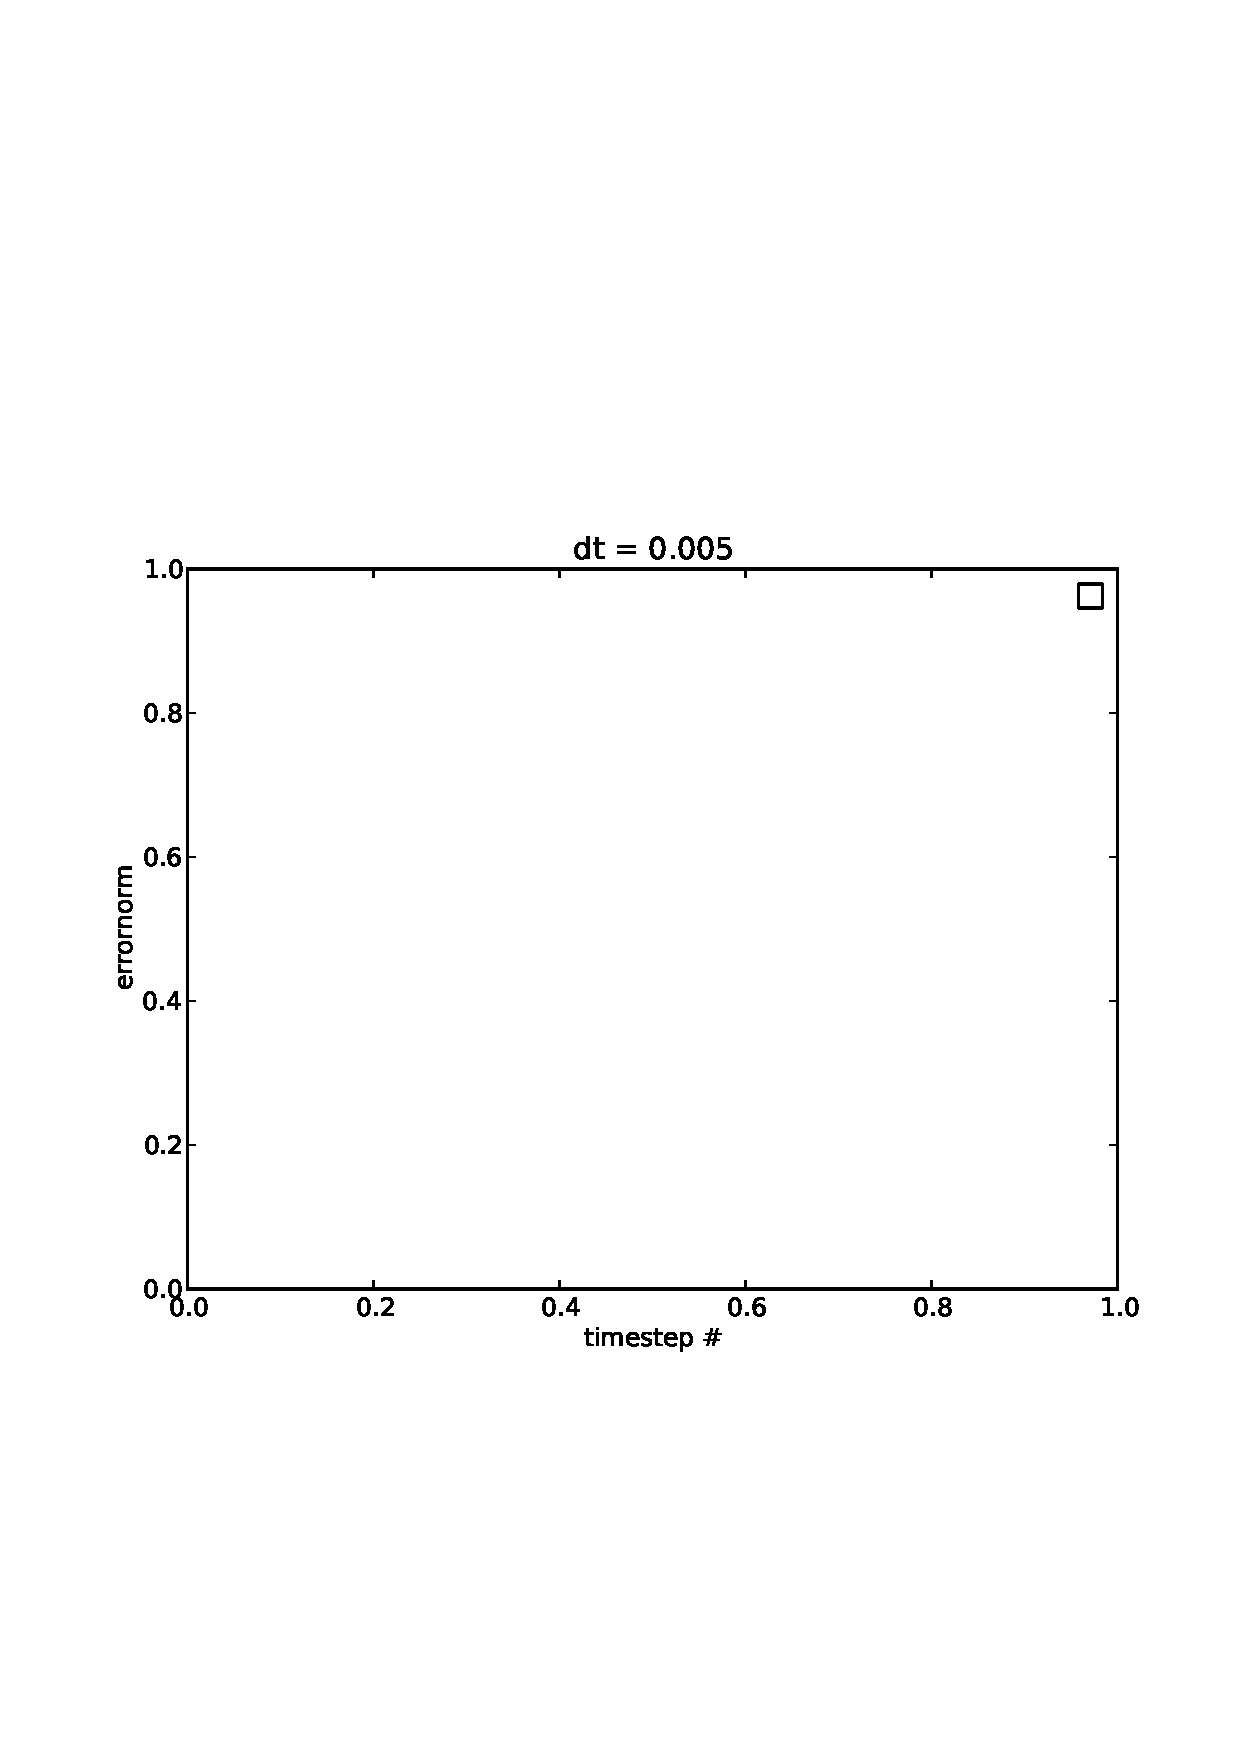
\includegraphics[width=\textwidth]{{../doc/results/experiment_02122013_1309_long_simulations_1d/results/deterministic_errorplot}.eps}
\caption{}
\label{errorplot_FE_walk_long:deterministic}
 \end{subfigure}
\caption[Errorplot, long simulation]{The deterministic error and the error from simulations with walkers for long simulations.}
\label{errorplot_FE_walk_long}
\end{figure}

\subsection{The effects of adding drift to the walkers}\label{effect_of_drift_on_walkers}

As shown in section \ref{random_walks_and_drift} adding drift to the walkers will modify our model to represent the convection diffusion equation (\ref{convection_diffusion_equation}) rather than the simple diffusion equation. 
In our analysis so far we have completely ignored the spatial truncation error because it is of second order, and the truncation error in time is of first order. 
When discretizing the convection diffusion equation however, we must take care to use an approximation to the first order spatial derivative that has a truncation error of second order. 

Otherwise the truncation error in this term will completely dominate seeing as $\Delta t<\Delta x$. 
We must also find a new stability criterion for the scheme. \\
As for now, the Leap-frog discretization will do (though it is not by far a perfect choice seeing as it is unstable). 
As a side note we can also note that the Neumann boundary condition will be very clear in this scheme. 
$\frac{\d C}{\d n} = 0 \implies \frac{\d C}{\d x} = 0 $ on the boundary, leading to $C_{-1} = C_{1}$ on the boundary and canceling the drift term on the boundary.
\begin{equation}\label{convection_diffusion_equation_leapfrog}
 C^{n+1} = \frac{D\Delta t}{\Delta x^2}\left(C^n_{i+1}-2C^n_i+C^n_{i-1}\right)-\frac{v\Delta t}{2\Delta x}\left(C^n_{i+1}-C^n_{i-1}\right) + C^n
\end{equation}
The truncation error for the first order derivative using the Leap-frog scheme is obtained as follows
\begin{align*}
 u(t,x+\Delta x) = u(t,x) + \frac{\d u(t,x)}{\d x}\Delta x + \frac{\d^2u(t,x)}{2\d x^2}\Delta x^2 +\mathcal{O}(\Delta x^3)\\
 u(t,x-\Delta x) = u(t,x) - \frac{\d u(t,x)}{\d x}\Delta x + \frac{\d^2u(t,x)}{2\d x^2}\Delta x^2 +\mathcal{O}(\Delta x^3)
\end{align*}
which we recognize as the same error we got from the second order spatial derivatives.\\
If we now do the same analysis as we have already done, by finding a manufactured solution to the convection diffusion equation, implementing a numerical scheme like \ref{convection_diffusion_equation_leapfrog} to solve it after and taking the error norm. \\
The error norm does not have to go as $\Delta t$, but it must be halved (approximately) if we halve $\Delta t$. 
Figure \ref{} shows two simulations of equation \ref{convection_diffusion_equation} for $D =1$ and $v=1$ compared to the manufactured solution \ref{manifactured_solution_1D} without adding walkers. 
Before the simulation we must find a source term so the manufactured solution will solve the equation.
\begin{align*}
 -\pi^2\exp\left(-\pi^2t\right)\cos\left(\pi x\right) &= -\pi^2D\exp\left(-\pi^2t\right)\cos\left(\pi x\right) + \pi v \exp\left(-\pi^2t\right)\sin\left(\pi x\right) + f(x,t)\\
 -\pi^2\cos\left(\pi x\right) &= \pi^2D\cos\left(\pi x\right) +\pi v \sin\left(\pi x\right) + \tilde{f}(x) \\
 \tilde{f}(x) &= -\pi\sin\left(\pi x\right)
\end{align*}
Where $f(x,t) = \exp\left(-\pi^2t\right)\tilde{f}(x)$.

\begin{figure}[H]
\centering
\begin{subfigure}[b]{0.48\textwidth}
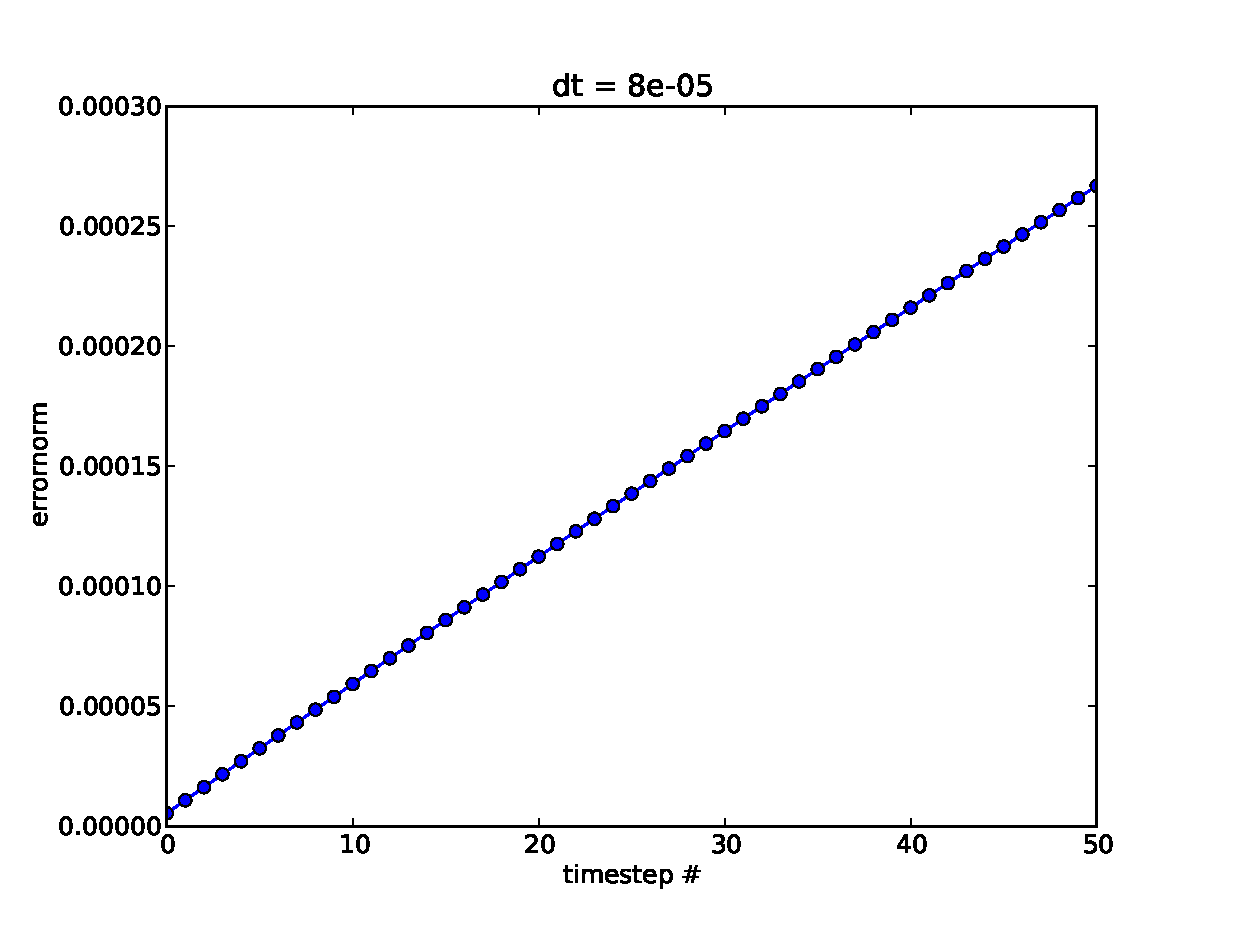
\includegraphics[width=\textwidth]{../doc/results/experiment_05112013_1235/results/deterministic_errorplot.eps}
\caption{}
\label{Verification_convection_diffusion:single_dt}
\end{subfigure}
\begin{subfigure}[b]{0.48\textwidth}
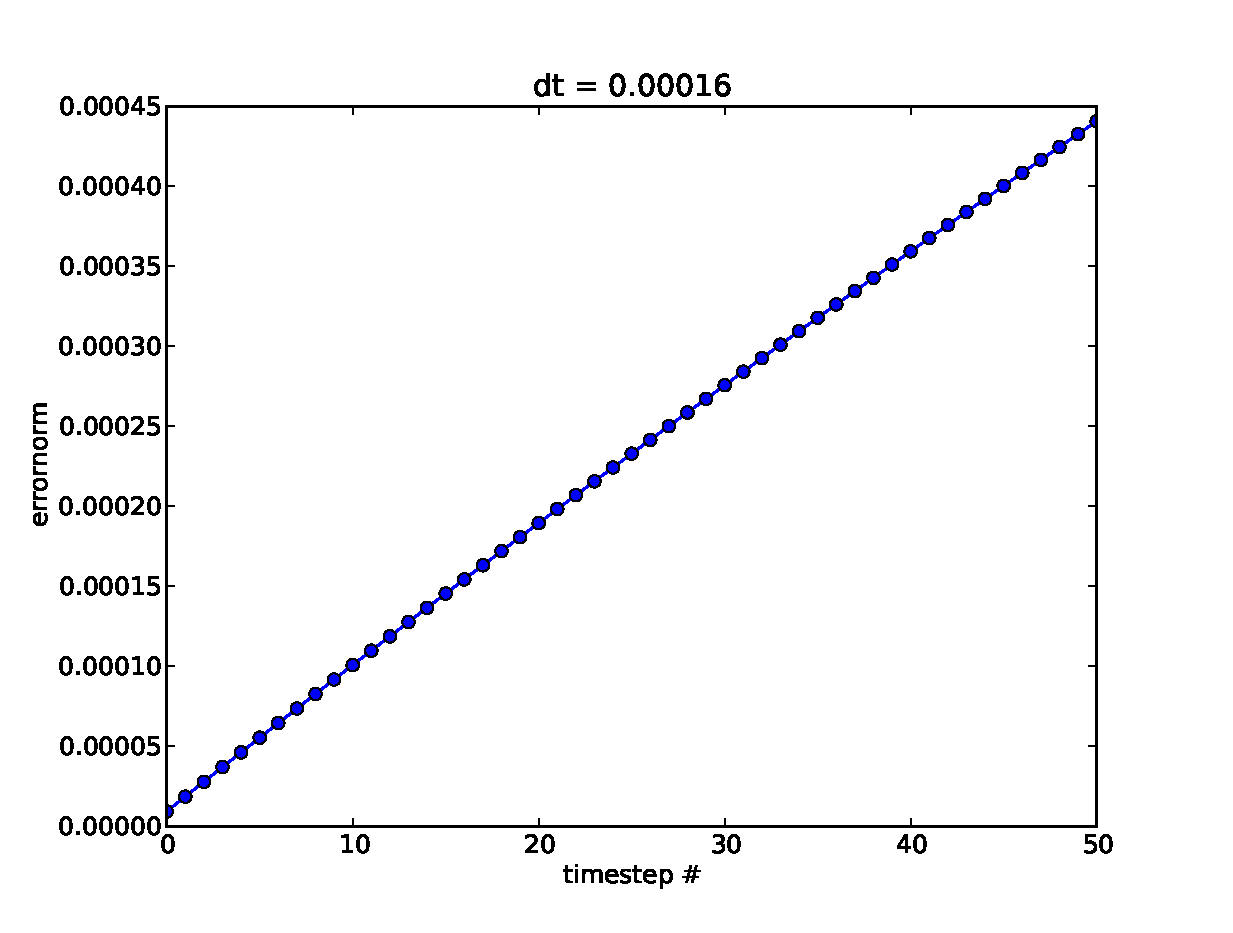
\includegraphics[width=\textwidth]{../doc/results/experiment_05112013_1234/results/deterministic_errorplot.eps}
\caption{}
\label{Verification_convection_diffusion:double_dt}
\end{subfigure}
\caption[Verification of Convection diffusion equation implementation]{Verification of Convection diffusion equation implementation}
\label{Verification_convection_diffusion}
\end{figure}

As we see from figure \ref{Verification_convection_diffusion} the error norm is halved when $\Delta t$ is roughly halved, just as we expected. It is also of the order of $\Delta t$, which is nice.  
We can then advance to testing the effect of adding an area of walkers for different values of $Hc$ as before. 
Note that we can no longer use the manufactured solution now if we wish to add drift to the walkers because we have forced the solution to fit the equation by tampering with the source term. 
The effect of
\begin{figure}[H]
\centering
\begin{subfigure}[b]{0.48\textwidth}
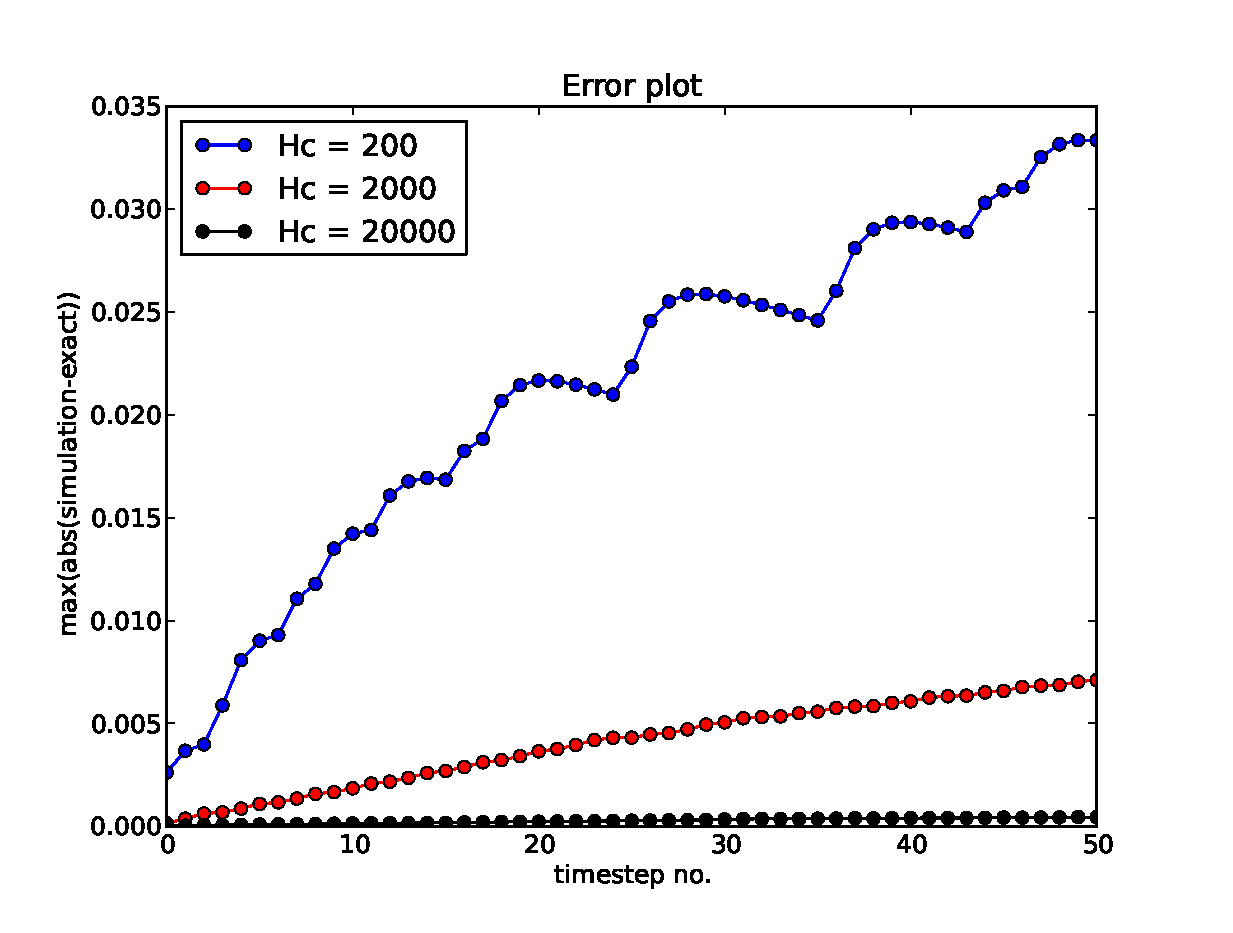
\includegraphics[width=\textwidth]{../doc/results/experiment_05112013_1237/results/errorplot.eps}
\caption{}
\label{Errortest_convection_diffusion_walkers:few_walkers}
\end{subfigure}
\begin{subfigure}[b]{0.48\textwidth}
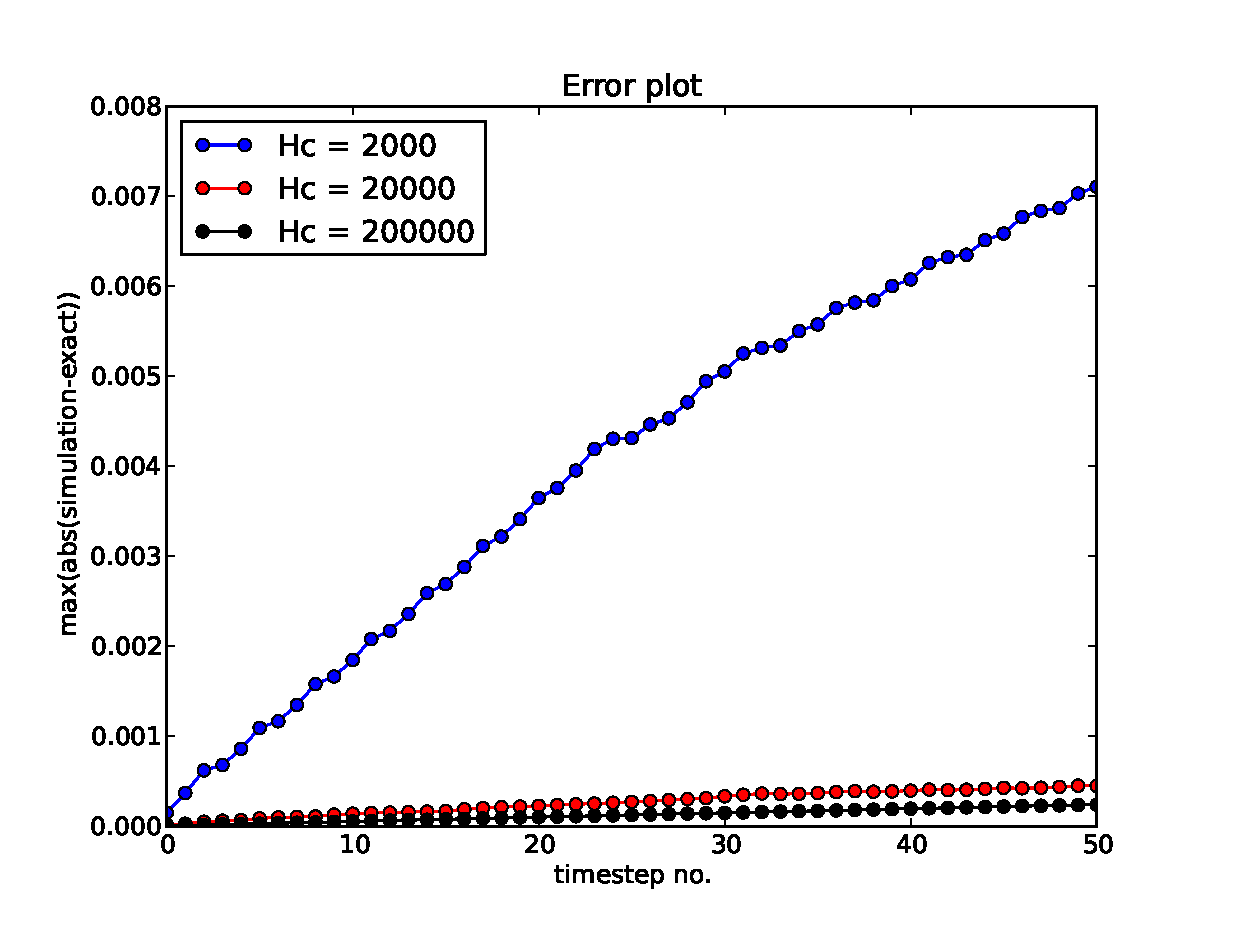
\includegraphics[width=\textwidth]{../doc/results/experiment_05112013_1239/results/errorplot.eps}
\caption{Adding more walkers still has the desired effect on the error, suggesting that the central limit theorem is at work behind the scenes.}
\label{Errortest_convection_diffusion_walkers:more_walkers}
\end{subfigure}
\caption[Adding walkers influenced by drift]{The figure shows the effect adding walkers influenced by drift has on the error. 
The drift term is the step length, which is quite large. The strangest thig is, however, that changing the direction of the drift has little effect on the error, suggesting that the drift term is completely wrong in relation to the steplength. $\Delta t =8e-5$}
\label{Errortest_convection_diffusion_walkers}
\end{figure}



\subsection{Anisotropic diffusion}

As we discussed in section \ref{random_walks_and_anisotropy} we should also be able to model diffusion where the diffusion constant is not a constant. 
The scheme we derived in section \ref{discretizing} already takes this into account, and so all we need to do is to add the drift term which was discussed in section \ref{effect_of_drift_on_walkers} to the scheme. 
Like before we should verify that the scheme solves the equation to the expected accuracy by using a manufactured solution \ref{manifactured_solution_1D} and tweaking the source term so this function solved the equation \ref{convection_diffusion_equation}. 
When $v=0$ and $D(x) = \pi x$ the source term becomes
\begin{align*}
 -\pi^2\exp\left(-\pi^2t\right)\cos\left(\pi x\right) &= -\pi\exp\left(-\pi^2t\right)\frac{\d}{\d x}\pi x\sin(\pi x) +f(x,t) \\
 -\pi^2\cos\left(\pi x\right) &= -\pi^2\left(\sin(\pi x) + \pi x\cos(\pi x)\right) +\tilde{f}(x) \\
 \tilde{f}(x) &= \pi^2\left(\sin(\pi x) +\cos(\pi x)(\pi x-1)\right)
\end{align*}
Once again $f(x,t) = \exp\left(-\pi^2t\right)\tilde{f}(x)$. Figure \ref{anisotropic_diffusion_verification} shows the error norm of the result of simulations of this equation with different values of $\Delta t$.

\begin{figure}[H]
\centering
\begin{subfigure}[b]{0.48\textwidth}
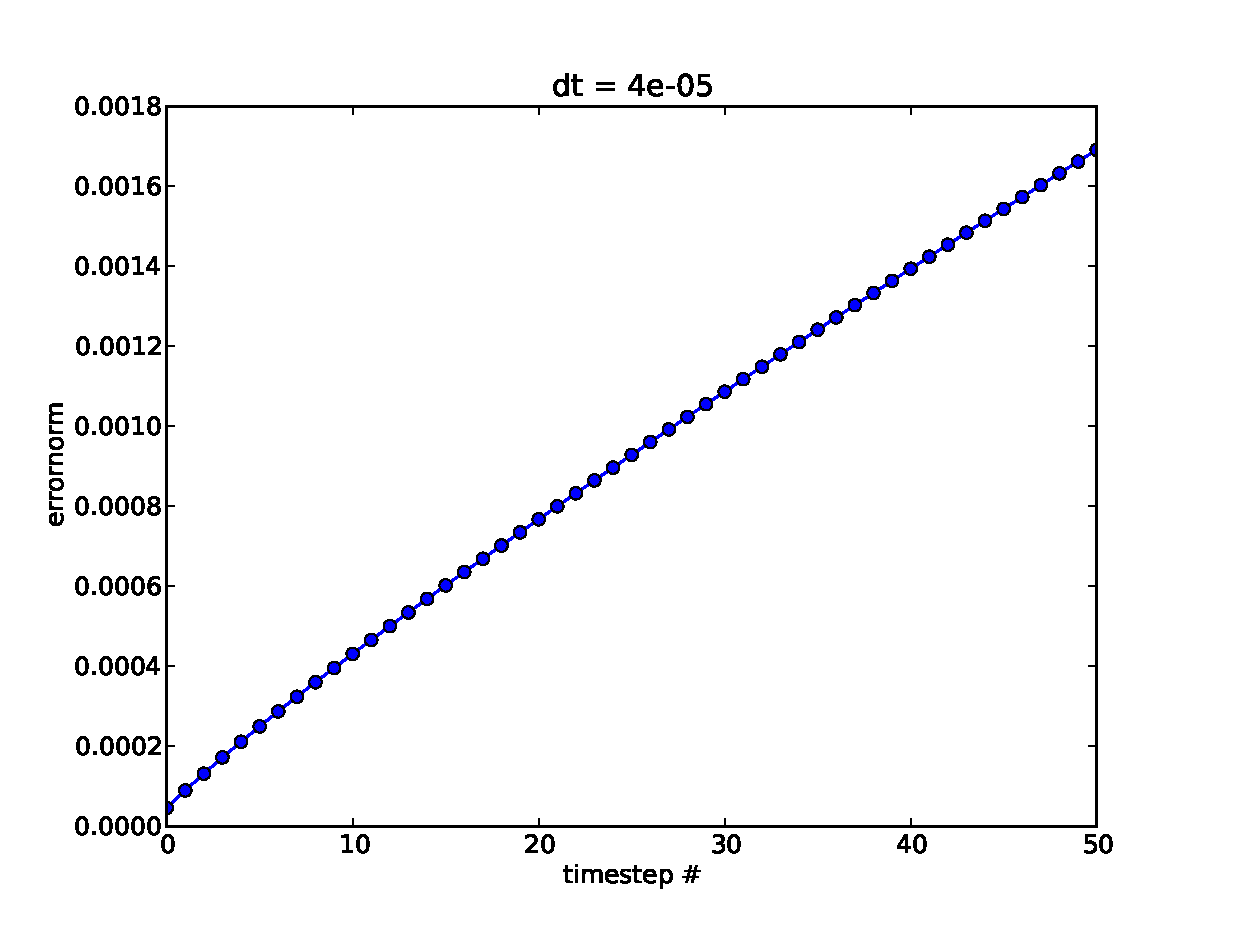
\includegraphics[width=\textwidth]{../doc/results/experiment_05112013_1303/results/deterministic_errorplot.eps}
\caption{}
\label{anisotropic_diffusion_verification:single_dt}
\end{subfigure}
\begin{subfigure}[b]{0.48\textwidth}
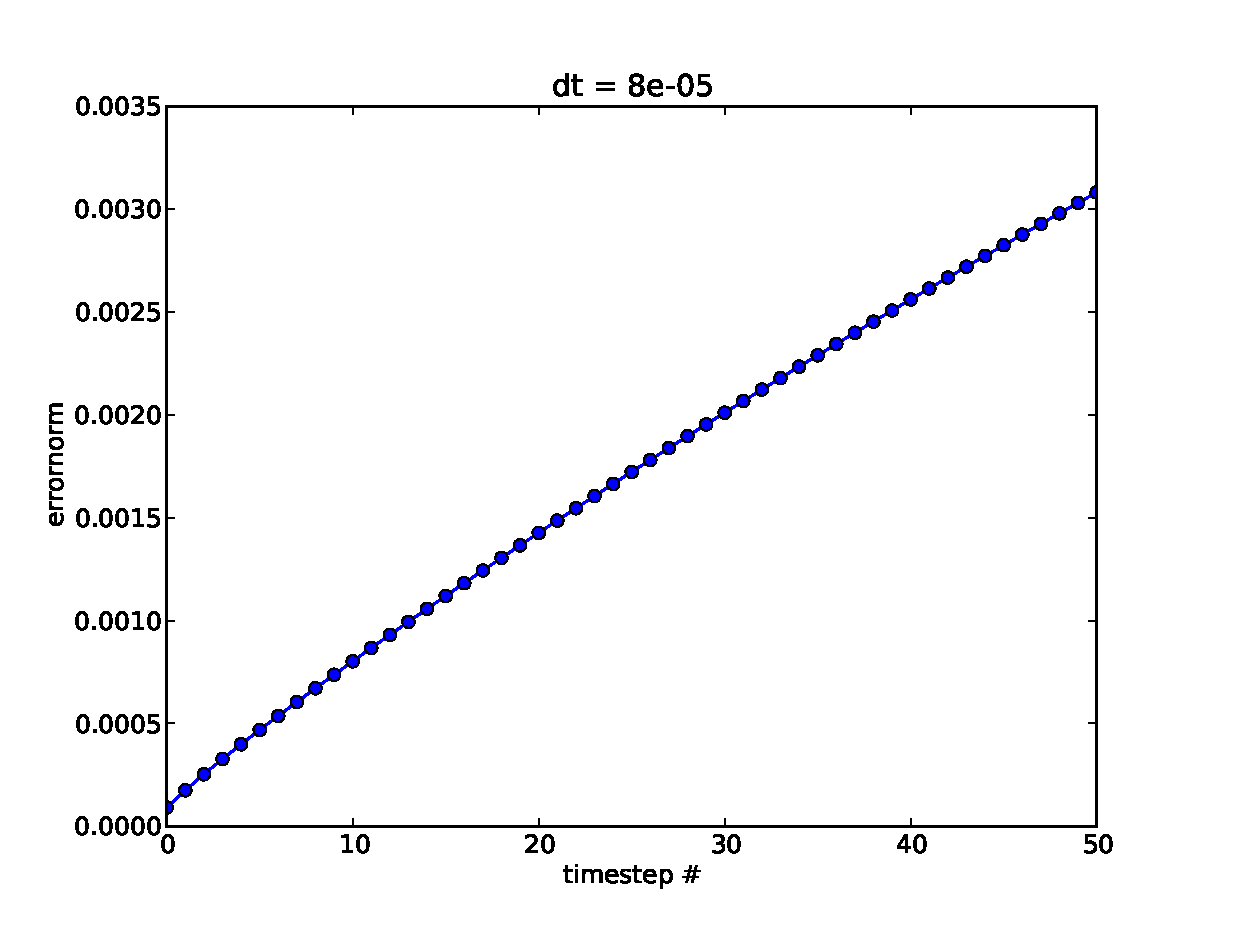
\includegraphics[width=\textwidth]{../doc/results/experiment_05112013_1304/results/deterministic_errorplot.eps}
\caption{}
\label{anisotropic_diffusion_verification:double_dt}
\end{subfigure}
\caption[Verification of anisotropic diffusion equation implementation]{Verification of anisotropic diffusion equation implementation}
\label{anisotropic_diffusion_verification}
\end{figure}
Again, the error is of the order of $\Delta t$ and is roughly halved by halving $\Delta t$.

\section{2D}
Doing the same tests is 2D gives slightly different results; adding a 2D walk-domain has an influence on the error, but a rather small one. 
This can, however be tweaked by increasing the conversion parameters.

\begin{equation}\label{initial_condition_2d_numex}
 u(x,y,t=0) = \cos(\pi x)\cos(\pi y)
\end{equation}

The exact numerical solution of the FE scheme can be found in equation \ref{exact_numerical_solution_2d}, and again we expect the scheme to be able to reproduce this to more or less machine precision. 
The result of a test simulation of this, using the initial condition in equation \ref{initial_condition_2d_numex}, is shown in figure \ref{exact_numerical_2d_n130}. 
Again, as in we did in 1d, we see that although the error is very small, and start out with machine precision, it does increase and even more than in the 1d case. 
This is \emph{probably} because of the terms we have do drop in the exact numerical solution due to overflow and so on, which accumulate in the numerical solution from the scheme. 
We should, in other words, be pleased that the error starts out with machine precision, and stays small for the ammount of time steps we can simulate and still have something to compare it with.

\begin{equation}\label{exact_numerical_solution_2d}
 u^{n+1} = \sum\limits^n_{i=0}{n\choose i}\left(D\Delta t\right)^i\left[2^{i-1}\cos(\pi x)\cos(\pi y)\left(\frac{(\cos(\pi\Delta x))^i}{\Delta x^{2i}} +\frac{(\cos(\pi\Delta y))^i}{\Delta y^{2i}}\right)\right]
\end{equation}

\begin{figure}[H]
 \centering
 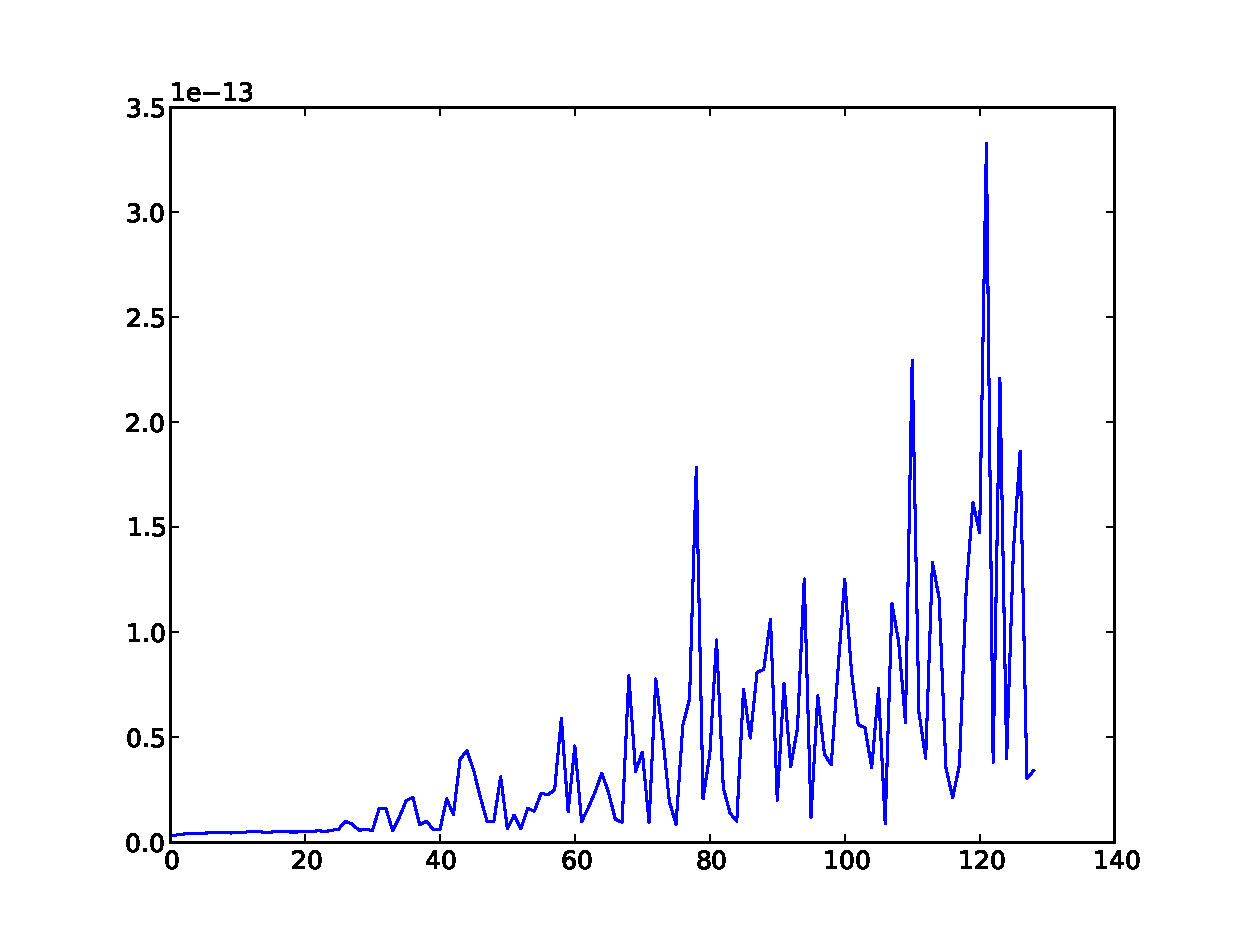
\includegraphics[scale=0.7]{Figures/exact_numerical_2d_n130.eps}
 \caption{Numerical solution from the FE scheme versus the exact numerical solution of the FE scheme in 2d. we have used a $\Delta t$ which is almost on the stability criterion, $\Delta t = \frac{\Delta x \Delta y}{5} = 8e-05$.}
 \label{exact_numerical_2d_n130}
\end{figure}

We can also do a convergence test, equal to the one we did in 1d, to check that the scheme converges to 1 (by equation \ref{convergence_rate_def}) for smaller $\Delta t$. 
The results of this test are shown in figure \ref{convergence_test_FE_2d} and it does converge nicely to one.

\begin{figure}[H]
\centering
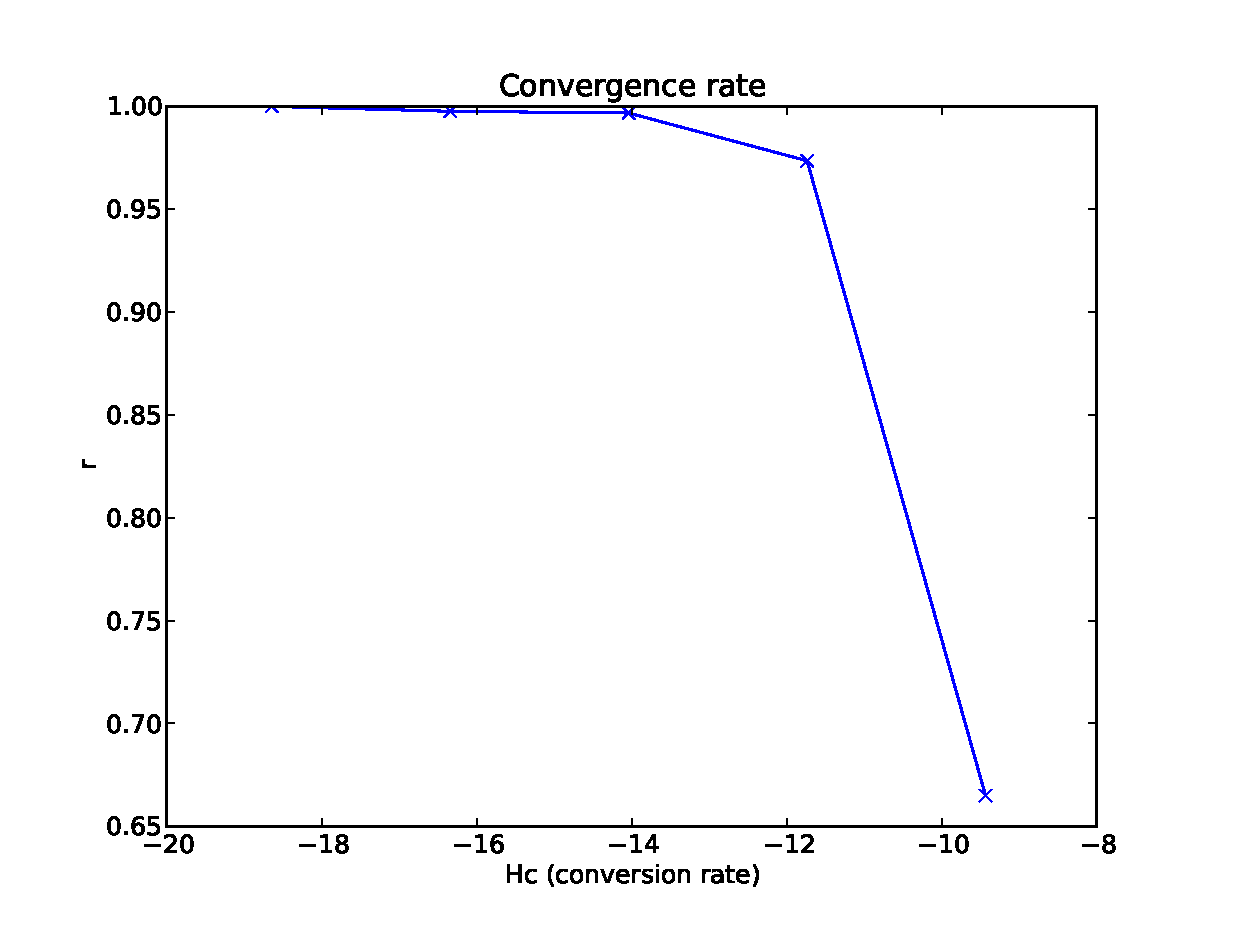
\includegraphics[scale=0.7]{../doc/results/experiment_29112013_1709/results/ConvergenceTest.eps}
\caption[Convergence test FE 2d]{Convergence test for the FE scheme in 2d using $\Delta t$ ranging from the stability criterion $\frac{\Delta x\Delta y}{5}$ to the same ratio divided by 100000 in increments of $10^{-1}$.}
\label{convergence_test_FE_2d}
\end{figure}

\subsection{Including random walks}

In the same way as in figure \ref{errorplot_FE1D_Walk_first_attemt} we can test the effect of introducing walkers in part of the mesh. 
In figure \ref{errorplot_FE1D_Walk_first_attemt_2d} we have more or less recreated the plot from the 1d case, only simulating for more time steps and with more walkers. 
First of all we note that we in 2d will need quite a lot more walkers than in 1d in order to get a decent error. 
Secondly, and more importantly, because we have done longer simulations, we notice that the error is completely dominated by the walkers. 
In the simulation in question the rectangle x0=0.4, x1=0.7 and y0=0.6 y1=0.7 has walkers on it.
The error does in fact seem to behave like a square root function. 
This is rather unnerving, and to check if this was the case in 1d as well a long simulation was run for a similar case. 
Figure \ref{errorplot_FE_walk_long} shows that the error in the long term behaves similarly to the error from the deterministic simulations, but with a \emph{much} larger amplitude. For the ``best'' case the maximum amplitude seems to be about a factor 100 times the deterministic one.

\begin{figure}[H]
\centering
\begin{subfigure}[b]{0.48\textwidth}
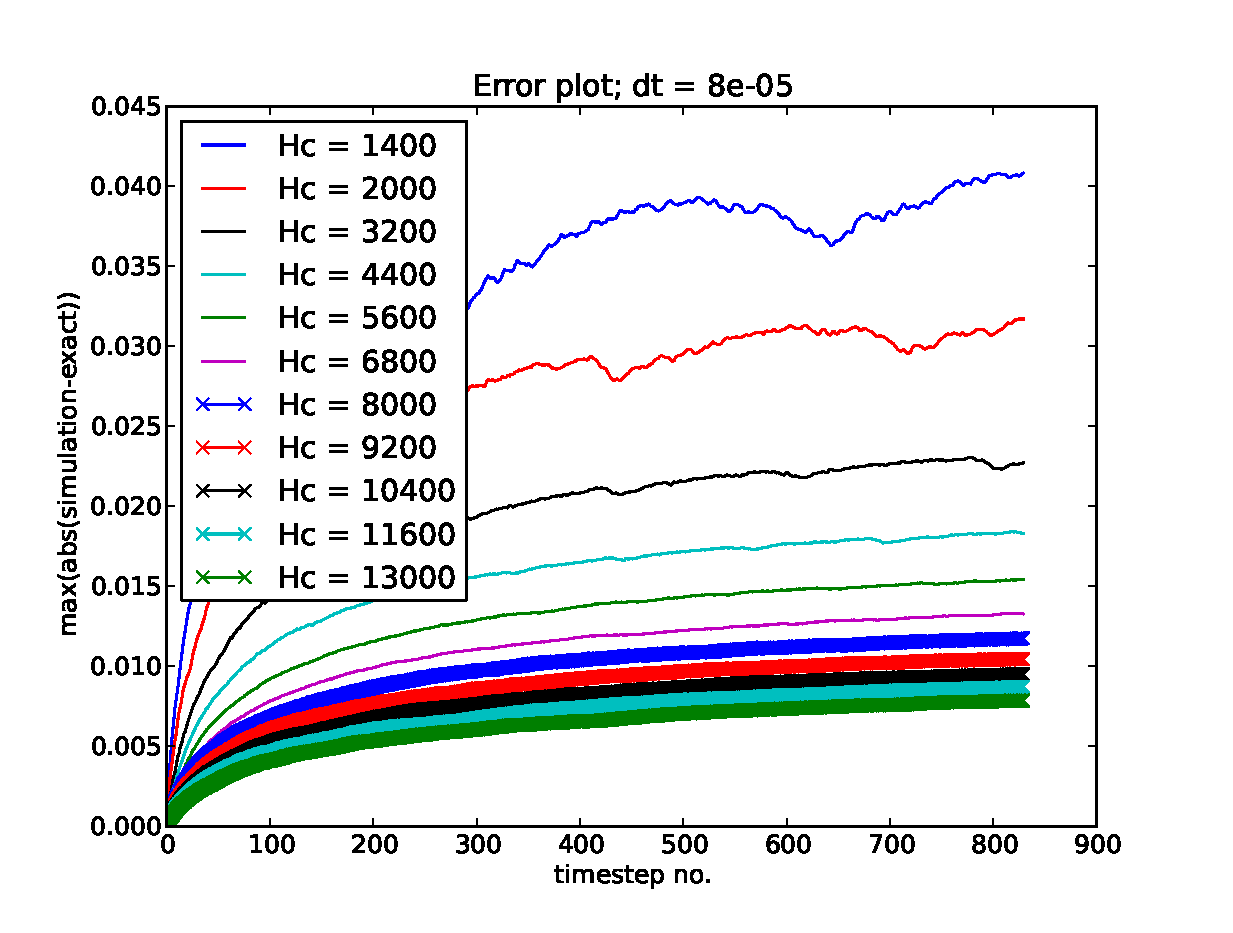
\includegraphics[width=\textwidth]{../doc/results/experiment_02122013_1229/results/errorplot.eps}
\caption{}
\label{errorplot_FE1D_Walk_first_attemt_2d:few_walkers}
\end{subfigure}
\begin{subfigure}[b]{0.48\textwidth}
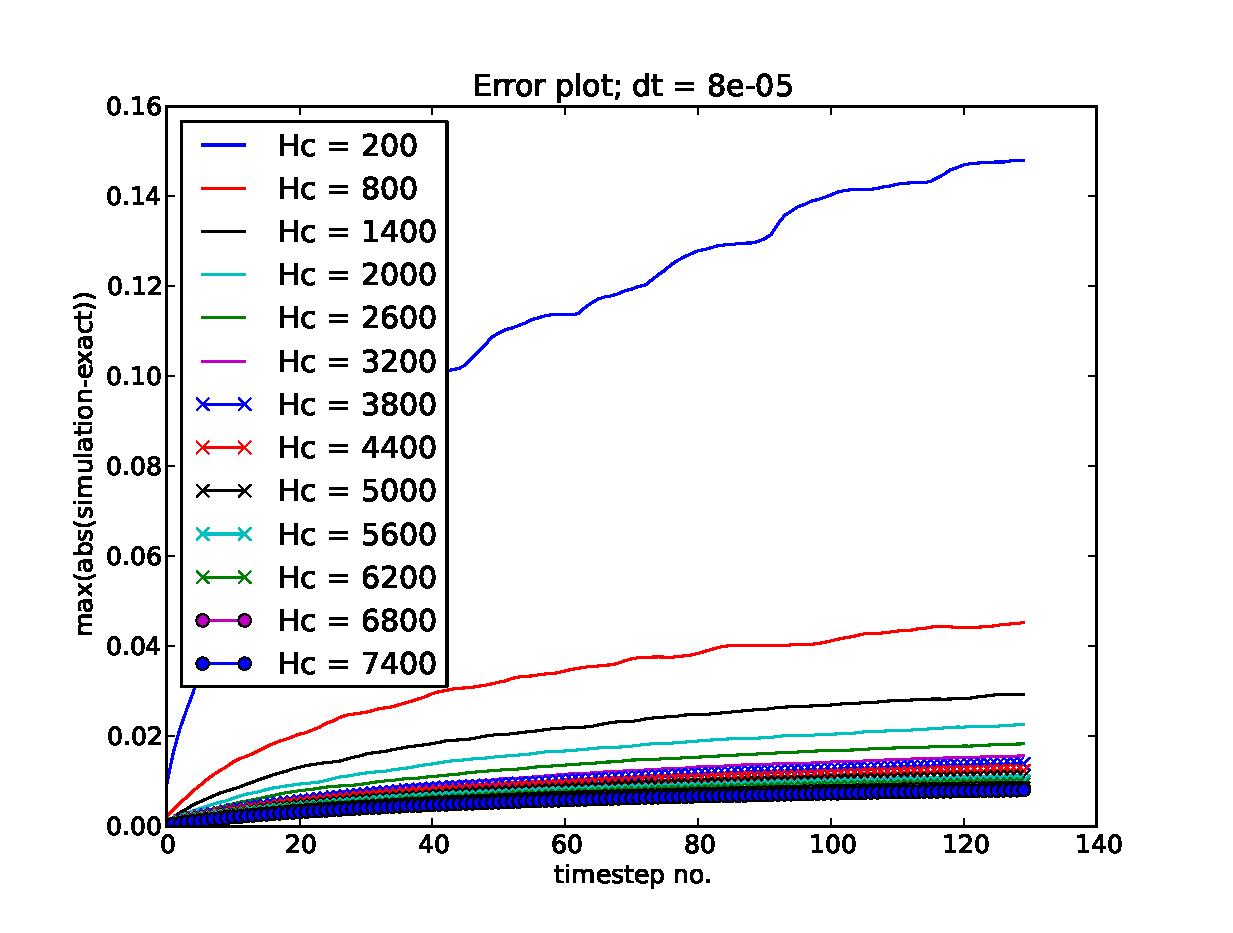
\includegraphics[width=\textwidth]{../doc/results/experiment_02122013_1223/results/errorplot.eps}
\caption{}
\label{errorplot_FE1D_Walk_first_attemt_2d:many_walkers}
\end{subfigure}
\caption[Verification of anisotropic diffusion equation implementation]{Verification of anisotropic diffusion equation implementation}
\label{errorplot_FE1D_Walk_first_attemt_2d}
\end{figure}


\section{Testing Random walks}\label{testing_random_walks}

To verify our implementation, and perhaps gain some new knowledge we will do some testing on the random walks implementation as well. 
This means that we have to find a solution of the diffusion equation \ref{simple_diffusion_equation} for an initial condition we can recreate with random walkers to the best possible precision. 
The absolute simplest initial condition to recreate is the Heaviside step function, defined in equation \ref{Heaviside_def}. 
\begin{equation}\label{Heaviside_def}
 H(x-a) = \begin{cases}
           1\;\;x\geq a\\
           0\;\;x<a
          \end{cases}
\end{equation}
We then solve the equation by separation of variables. We have
\begin{align*}
 \frac{\d u}{\d t} = D\frac{\d^2 u}{\d x^2};\;\; \frac{\d u(0,t)}{\d x} = \frac{\d u(1,t)}{\d x} = 0 \\
 u(x,0) = H\left(x-\frac{1}{2}\right);\;\; D = 1
\end{align*}
and
\begin{align*}
 u(x,t) = F(x)T(t) \implies \frac{T'(t)}{T(t)} = \frac{F''(x)}{F(x)}
\end{align*}
where the primes denotes the respective derivatives. We separate the equation using a separation constant $\lambda$
\begin{align*}
 T'(t)-\lambda T(t) = 0 \implies T(t) = C\exp(\lambda t)\\
 F''(x) -\lambda F(x) = 0 \implies F(x) = C_1\exp(\sqrt{\lambda}x) + C_2\exp(-\sqrt{\lambda}x)
\end{align*}
Where $C$, $C_1$ and $C_2$ are arbitrary constants. 
Choosing $\lambda = -\mu^2$ lets us rewrite the spatial solution in terms of sines and cosines
\begin{equation*}
 F(x) = a\cos(\mu x) + b\sin(\mu x)
\end{equation*}
The boundary conditions gives us 
\begin{align*}
 F'(0)T(t) = F'(1)T(t) = 0
\end{align*}
Since the time dependent solution cannot be exactly zero, the first derivative of the spatial solution must be zero
\begin{align*}
 F'(x) &= -a\mu\sin(\mu x) + b\mu\cos(\mu x) \\
 F'(0) &= -a \mu\sin(0) + b\mu\cos(\mu x) = b\mu\cos(\mu x) \implies b=0 \\
 F(1) &= a\cos(\mu) \implies \mu = n\pi
\end{align*}
Telling us that a Fourier series in cosines is the solution to the equation, and it will look like this.
\begin{equation}
 u(x,t) = a_0 + \sum\limits_{n=1}^\infty a_n\exp\left(-(n\pi)^2t\right)\cos(n\pi x)
\end{equation}

The coefficients are found by approximating the initial condition
\begin{align*}
 a_0 &= \int\limits_0^1H(x-0.5)dx = \frac{1}{2} \\
 a_n &= 2\int\limits_0^1H(x-0.5)\cos(n\pi x)dx = 2\int\limits_{0.5}^1\cos(n\pi x)dx \\
 &= \frac{2}{n\pi}\left[sin(n\pi x)\right]_{0.5}^1 = \frac{2}{n\pi}\sin(n\pi) - \sin(\frac{n\pi}{2}) \\
 a_n &= \frac{2\sin(\frac{n\pi}{2})}{n\pi}
\end{align*}
which gives us the final solution
\begin{equation}
 u(x,t) = \frac{1}{2} + \sum\limits_{n=1}^\infty \frac{2\sin(\frac{n\pi}{2})}{n\pi}\exp\left(-(n\pi)^2t\right)\cos(n\pi x)
\end{equation}

We can now perform a convergence test to find the convergence rate for the random walkers, this is the order the error of the scheme goes as and it is defined in equation \ref{convergence_rate_def}. 
We will modify it slightly by testing for the number of walkers rather than the time step. 
We must also use another error estimate $E_i$ which gives us one number for each simulation. 
The candidates are either the maximum of the error we are already using, or an integrated error.

\begin{equation}\label{convergence_rate_def}
 r = \frac{\ln(E_{i+1}/E_i)}{\ln(\Delta t_{i+1}/\Delta t_i)}
\end{equation}

Using the maximum of the error measure already in use, we have tested the convergence rate measure for the following measures of Hc:
\begin{lstlisting}
 Hc = [100,500,1000,5000,10000,50000]
\end{lstlisting}
Meaning that the largest value of Hc we will get an estimate for is $Hc = 10000$. 
The convergence test suggests that the convergence rate for random walks follows the proportionality in equation \ref{convergence_rate_RW}. 
This relation tells us just what we have been expecting the whole time; while increasing the number of walkers will reduce the error, the convergence is slow. 
Should we wish to do so, we can force the error to $\mathcal{O}(\Delta t^2)$, but this will be extremely inefficient. In fact we can find the relation as $Hc\sim\Delta t^{-2}$ for $err\sim\mathcal{O}(\Delta t)$, and $Hc\sim\Delta t^{-4}$ for $err\sim\mathcal{O}(\Delta t^2)$. Clearly we will have enough trouble for the simpler cases.

\begin{equation}\label{convergence_rate_RW}
err \propto Hc^{\frac{-1}{2}}
\end{equation}


\begin{figure}[H]
 \centering
 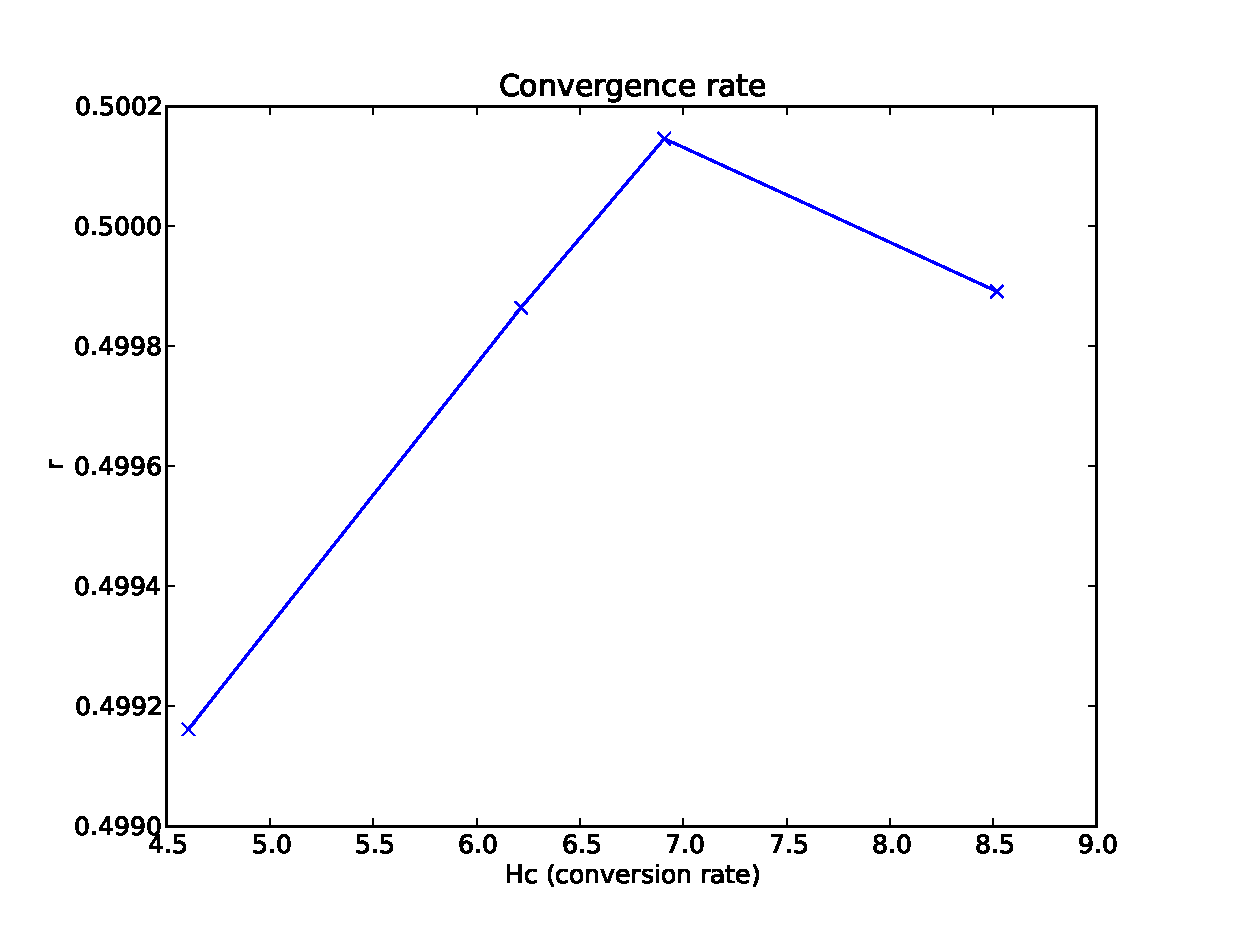
\includegraphics[scale=0.7]{../doc/results/experiment_27112013_0837/resultsConvergenceTest.eps}
 \caption[Convergence test RW]{A convergence test for the isotropic random walk implementation using different conversion factors, Hc. The x axis (conversion rate) is log transformed and ranges from 100 to 50000 in real numbers.}
 \label{ConvergenceTestRW}
\end{figure}
\begin{figure}[H]
 \centering
 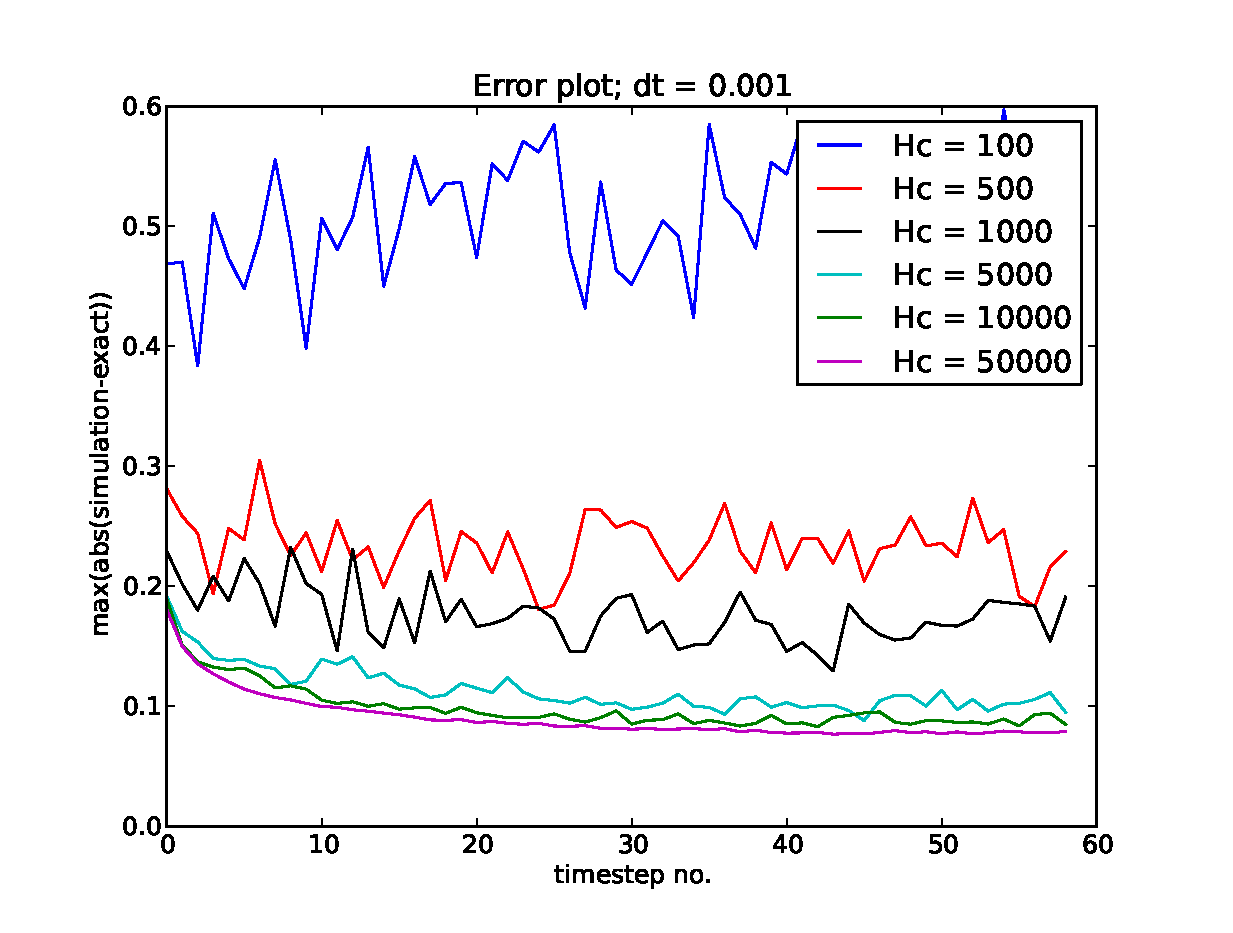
\includegraphics[scale=0.7]{../doc/results/experiment_24112013_1525/results/errorplot.eps}
 \caption[Error plot RW]{A ``normal'' error plot for the same simulation as in figure \ref{ConvergenceTestRW}. The $\Delta t$ in question is used to couple the RW simulation and the exact solution. For each $\Delta t$ the RW simulation does 100 steps with a step length calculated from equation \ref{steplength}}
\end{figure}

